\documentclass[11pt,a4paper]{report}

% ============================================================
% PAKETE
% ============================================================
\usepackage[utf8]{inputenc}
\usepackage[T1]{fontenc}
\usepackage[ngerman]{babel}
\usepackage{amsmath, amssymb, amsthm}
\usepackage{geometry}
\usepackage{booktabs}
\usepackage{array}
\usepackage{longtable}
\usepackage{hyperref}
\usepackage{xcolor}
\usepackage{listings}
\usepackage{enumitem}
\usepackage{tcolorbox}
\usepackage{graphicx}
\usepackage{float}
\usepackage{microtype}
\usepackage{lmodern}
\usepackage{setspace}
\usepackage{subcaption}
\usepackage{csquotes}
\usepackage[backend=biber, style=numeric, sorting=nyt, maxnames=3]{biblatex}
\usepackage{fancyhdr}
\usepackage{emptypage}
\usepackage{caption}
\usepackage{multirow}

\addbibresource{references.bib}
\graphicspath{{figures/}}

% ============================================================
% LAYOUT
% ============================================================
\geometry{
a4paper,
top=2.5cm, bottom=2.5cm,
left=3.0cm, right=2.5cm
}
\setlength{\parskip}{6pt}
\setlength{\parindent}{0pt}
\onehalfspacing

\pagestyle{fancy}
\fancyhf{}
\fancyhead[L]{\small\nouppercase{\leftmark}}
\fancyhead[R]{\small\textit{L2ML-Fitting-Tool -- Methodendokumentation}}
\fancyfoot[C]{\thepage}
\renewcommand{\headrulewidth}{0.4pt}

\setcounter{secnumdepth}{3}
\setcounter{tocdepth}{3}

% ============================================================
% FARBEN & BOXEN
% ============================================================
\definecolor{boxblue}{RGB}{220,235,250}
\definecolor{boxgreen}{RGB}{220,245,220}
\definecolor{codegray}{RGB}{245,245,245}
\definecolor{codegreen}{rgb}{0,0.5,0}
\definecolor{codepurple}{rgb}{0.5,0,0.5}

\tcbuselibrary{skins, breakable}

\newtcolorbox{analogiebox}[1][]{
colback=boxblue, colframe=blue!50!black,
title=Analogie, fonttitle=\bfseries,
breakable, #1
}

\newtcolorbox{merkbox}[1][]{
colback=boxgreen, colframe=green!40!black,
title=Merksatz, fonttitle=\bfseries,
breakable, #1
}

\newtcolorbox{hinweisbox}[1][]{
colback=yellow!15, colframe=orange!70!black,
title=Hinweis, fonttitle=\bfseries,
breakable, #1
}

% ============================================================
% LISTINGS
% ============================================================
\lstset{
backgroundcolor=\color{codegray},
basicstyle=\ttfamily\small,
breaklines=true,
captionpos=b,
commentstyle=\color{codegreen},
keywordstyle=\color{blue}\bfseries,
stringstyle=\color{codepurple},
numbers=left,
numberstyle=\tiny\color{gray},
frame=single,
rulecolor=\color{gray!40},
tabsize=4,
showstringspaces=false
}

% ============================================================
% HYPERREF
% ============================================================
\hypersetup{
colorlinks=true,
linkcolor=blue!60!black,
urlcolor=blue!60!black,
citecolor=blue!60!black,
pdftitle={Vergleich von Regressionsverfahren im maschinellen Lernen},
pdfauthor={heinzl75},
pdfsubject={HILOMOT, LOLIMOT, MLP, SVR, GPR, L2ML-Fitting-Tool}
}

\title{%
\vspace{-1.5cm}%
\rule{\linewidth}{0.5mm}\\[8pt]
{\LARGE\bfseries Vergleich von Regressionsverfahren\\[6pt]
im maschinellen Lernen}\\[8pt]
{\large HILOMOT, LOLIMOT, MLP, SVR und GPR\,--\\[4pt]
Theorie, Implementierung und Vergleich\\
anhand des L2ML-Fitting-Tool}\\[8pt]
\rule{\linewidth}{0.5mm}\\[20pt]
{\large Technische Dokumentation}
}
\author{}
\date{\today}

\begin{document}

% ============================================================
% TITELSEITE
% ============================================================
\maketitle
\thispagestyle{empty}
\vspace{3cm}

\begin{center}
{\large\bfseries Kurzfassung}
\end{center}
\begin{quote}
Diese technische Dokumentation gibt eine umfassende Einf\"{u}hrung in f\"{u}nf Regressionsverfahren
des maschinellen Lernens: HILOMOT, LOLIMOT, MLP, SVR und GPR.
Alle Methoden werden theoretisch hergeleitet, ihre Python-Implementierung in scikit-learn sowie
der Bezug zur MATLAB LMNTool-Toolbox erl\"{a}utert und anhand eines realen Datensatzes
(Tilt Angle in Abh\"{a}ngigkeit von Scherkraft und Normalkraft) direkt verglichen.
Die Dokumentation enth\"{a}lt Inhaltsverzeichnis, Abbildungsverzeichnis, Tabellenverzeichnis,
Quellenangaben sowie eine Diskussion und Zusammenfassung.
\end{quote}

\vfill
\begin{center}
{\small Erstellt mit \LaTeX{} und Biber/biblatex. Abbildungen aus dem L2ML-Fitting-Tool.}
\end{center}

\clearpage

% ============================================================
% VERZEICHNISSE
% ============================================================
\pagenumbering{roman}
\tableofcontents
\clearpage
\listoffigures
\addcontentsline{toc}{chapter}{Abbildungsverzeichnis}
\clearpage
\listoftables
\addcontentsline{toc}{chapter}{Tabellenverzeichnis}
\clearpage
\pagenumbering{arabic}

% ============================================================
\chapter{Einleitung}
% ============================================================

\section{Motivation und Hintergrund}

Die Modellierung nichtlinearer Zusammenh\"{a}nge zwischen Messgr\"{o}ssen ist eine der zentralen
Aufgaben der modernen Ingenieurswissenschaften. In der Praxis werden physikalische Systeme --
von Verbrennungsmotoren \"{u}ber Robotergelenke bis hin zu chemischen Reaktoren -- durch
Messdaten charakterisiert, aus denen ein mathematisches Modell abgeleitet werden soll. Dieses
Vorgehen wird als \emph{datengetriebene Modellbildung} oder \emph{System Identification}
bezeichnet \cite{nelles2001}.

Klassische lineare Modelle sto\ss{}en bei stark nichtlinearen Systemen schnell an ihre Grenzen.
Auf der anderen Seite sind rein \emph{black-box}-Verfahren wie tiefe neuronale Netze zwar
leistungsf\"{a}hig, bieten aber wenig Einblick in die innere Struktur -- ein erheblicher Nachteil
in sicherheits- oder normrelevanten Anwendungen.

\emph{Lokale Modellnetze} (LMN) repr\"{a}sentieren in diesem Spannungsfeld einen attraktiven
Mittelweg: Sie zerlegen den Eingangsraum in Teilbereiche, in denen jeweils ein einfaches
lineares Modell gilt. Der Ansatz ist interpretierbar und gleichzeitig flexibel genug f\"{u}r
stark nichtlineare Kennlinien \cite{nelles2001, murray1998}.

Neben den LMN-Verfahren werden in dieser Dokumentation drei weitere etablierte Methoden
untersucht: das Multilayer Perceptron (MLP) als Vertreter der neuronalen Netze \cite{goodfellow2016},
die Support Vector Regression (SVR) \cite{vapnik1998} und die Gaussian Process Regression (GPR)
\cite{rasmussen2006}. Alle f\"{u}nf Methoden sind im \emph{L2ML-Fitting-Tool} implementiert
und k\"{o}nnen direkt miteinander verglichen werden.

\section{Ziel und Aufbau der Dokumentation}

Diese Dokumentation verfolgt vier Hauptziele:

\begin{enumerate}
\item \textbf{Theorie:} Die mathematischen Grundlagen aller f\"{u}nf Verfahren werden
      aus ersten Prinzipien hergeleitet, mit Bezug zu einschl\"{a}giger Fachliteratur
      und Online-Dokumentationen (MATLAB~\cite{matlab_gpr,matlab_svr,matlab_neural},
      scikit-learn~\cite{sklearn_mlp,sklearn_svr,sklearn_gpr}).

\item \textbf{Implementierung:} Die konkrete Umsetzung in zwei Werkzeugen wird beschrieben:
      im Python-Tool \emph{L2ML-Fitting-Tool} (f\"{u}nf-Methoden-Vergleich) sowie in
      \emph{MeinWindowLMNTool} (MATLAB-App-Designer-basiertes Trainingswerkzeug f\"{u}r
      HILOMOT/LOLIMOT), einschlie\ss{}lich aller relevanten Hyperparameter und ihrer Wirkung.

\item \textbf{Vergleich:} Alle Methoden werden auf demselben Datensatz trainiert und mit
      einheitlichen G\"{u}tekriterien verglichen.

\item \textbf{Empfehlung:} Auf Basis des Vergleichs werden Entscheidungshilfen f\"{u}r die
      Methodenwahl in der Praxis abgeleitet.
\end{enumerate}

Der Aufbau der Dokumentation:

\begin{description}
\item[Kapitel~2] Mathematische Grundlagen der Regression: G\"{u}tekriterien, Kreuzvalidierung,
    Bias-Varianz-Dilemma.
\item[Kapitel~3] Lokale Modellnetze -- allgemeine Theorie (LMN, Partition of Unity,
    G\"{u}ltigkeitsfunktionen).
\item[Kapitel~4] LOLIMOT -- achsenparallele Splits, Algorithmus, Hyperparameter.
\item[Kapitel~5] HILOMOT -- oblique Splits, Baumstruktur, Winkeloptimierung.
\item[Kapitel~6] MLP -- Architektur, Backpropagation, Aktivierungsfunktionen.
\item[Kapitel~7] SVR -- $\varepsilon$-Margin, Kernel-Trick, RBF-Kernel.
\item[Kapitel~8] GPR -- Gau\ss{}prozesse, Kovarianzfunktionen, Bayes'sche Inferenz.
\item[Kapitel~9] L2ML-Tool -- Python-Vergleichswerkzeug (L2ML-Fitting-Tool) und MATLAB-App-Designer-Werkzeug (MeinWindowLMNTool) f\"{u}r HILOMOT/LOLIMOT: Datenimport, Parameter, Visualisierungen, Export.
\item[Kapitel~10] Vergleich aller f\"{u}nf Methoden.
\item[Kapitel~11] Diskussion.
\item[Kapitel~12] Zusammenfassung und Ausblick.
\end{description}

\section{Verwendeter Datensatz}

Der in dieser Dokumentation durchg\"{a}ngig verwendete Datensatz beschreibt den \emph{Tilt Angle}
(Neigungswinkel) in Abh\"{a}ngigkeit zweier Eingansgr\"{o}\ss{}en:

\begin{itemize}
\item $x_1$: \textbf{Shear Force} (Scherkraft)
\item $x_2$: \textbf{Normal Force} (Normalkraft)
\item $y$: \textbf{Tilt Angle} (Neigungswinkel, Zielgr\"{o}\ss{}e)
\end{itemize}

\begin{figure}[H]
\centering
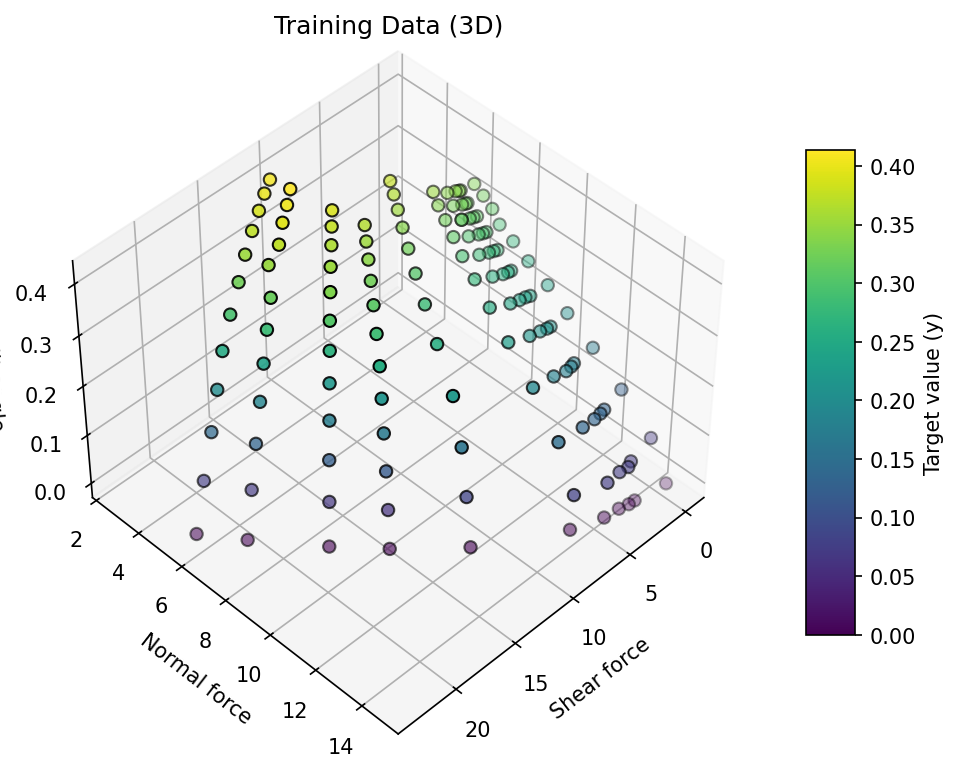
\includegraphics[width=0.68\textwidth]{training_data_3d.png}
\caption{3D-Ansicht der Trainingsdaten nach dem CSV-Import im L2ML-Fitting-Tool. Die Zielgr\"{o}\ss{}e $y$
(Tilt Angle) ist als farbcodierte H\"{o}he \"{u}ber den Eingansgr\"{o}\ss{}en $x_1$ (Shear Force) und
$x_2$ (Normal Force) aufgetragen (blau\,$=$\,kleine Werte, rot\,$=$\,gro\ss{}e Werte).}
\label{fig:training_data}
\end{figure}

Der Datensatz weist eine glatte, nichtlineare Abh\"{a}ngigkeit der Zielgr\"{o}\ss{}e von beiden
Eingansgr\"{o}\ss{}en auf und eignet sich damit gut f\"{u}r den Methodenvergleich. Die Daten wurden
im L2ML-Fitting-Tool als CSV-Datei importiert (Spaltenreihenfolge: $y$, $x_1$, $x_2$) und f\"{u}r alle
f\"{u}nf Verfahren auf identischer Basis verwendet.

% ============================================================
\chapter{Mathematische Grundlagen der Regression}
% ============================================================

\section{Was ist Regression?}

Unter \emph{Regression} versteht man die statistische Aufgabe, aus einem Datensatz
$\mathcal{D} = \{(\mathbf{x}_i, y_i)\}_{i=1}^N$ eine Funktion
$\hat{f}: \mathbb{R}^n \to \mathbb{R}$ zu sch\"{a}tzen, die f\"{u}r neue Eingangsvektoren
$\mathbf{x}^*$ eine m\"{o}glichst genaue Vorhersage des zugeh\"{o}rigen Ausgangswerts $y^*$
liefert \cite{bishop2006}.

Das allgemeine Regressionsmodell lautet:
\begin{equation}
y_i = f(\mathbf{x}_i) + \varepsilon_i, \qquad \varepsilon_i \sim \mathcal{N}(0, \sigma^2)
\label{eq:regression_model}
\end{equation}
wobei $\varepsilon_i$ das Messrauschen repr\"{a}sentiert und als normalverteilt angenommen wird.
Das Ziel ist, $f$ durch $\hat{f}$ so zu approximieren, dass der Erwartungswert eines gew\"{a}hlten
Verlustma\ss{}es minimiert wird.

Die Komplexit\"{a}t des Regressionsmodells muss an die Komplexit\"{a}t der zugrunde liegenden
Funktion $f$ angepasst werden. Ist das Modell zu einfach, wird die Funktion nicht gut
gen\"{u}gend beschrieben (\emph{Underfitting}). Ist das Modell zu komplex, lernt es das Rauschen
in den Trainingsdaten auswendig (\emph{Overfitting}) \cite{hastie2009}.

\section{G\"{u}tekriterien}
\label{sec:guetekriterien}

Zur Bewertung der Modellg\"{u}te werden im L2ML-Fitting-Tool die folgenden standardisierten Ma\ss{}e
verwendet \cite{hastie2009,bishop2006}:

\subsection{Mittlerer quadratischer Fehler (MSE)}

\begin{equation}
\mathrm{MSE} = \frac{1}{N}\sum_{i=1}^{N}\bigl(y_i - \hat{y}_i\bigr)^2
\label{eq:mse}
\end{equation}

Der MSE bewertet gro\ss{}e Abweichungen \"{u}berproportional (quadratisch). Er ist in den Einheiten
$[y]^2$ angegeben, was die direkte Interpretation erschwert. F\"{u}r Optimierung und Verlust-
funktionen wird MSE jedoch h\"{a}ufig bevorzugt.

\subsection{Mittlerer absoluter Fehler (MAE)}

\begin{equation}
\mathrm{MAE} = \frac{1}{N}\sum_{i=1}^{N}\bigl|y_i - \hat{y}_i\bigr|
\label{eq:mae}
\end{equation}

Der MAE ist robuster gegen\"{u}ber Ausrei\ss{}ern als der MSE und in denselben Einheiten wie $y$.

\subsection{Wurzel des MSE (RMSE)}

\begin{equation}
\mathrm{RMSE} = \sqrt{\mathrm{MSE}} = \sqrt{\frac{1}{N}\sum_{i=1}^{N}(y_i-\hat{y}_i)^2}
\end{equation}

Der RMSE ist in denselben Einheiten wie $y$ und damit intuitiver als der MSE.

\subsection{Bestimmtheitsma\ss{} $R^2$}

\begin{equation}
R^2 = 1 - \frac{\sum_{i=1}^{N}(y_i-\hat{y}_i)^2}{\sum_{i=1}^{N}(y_i-\bar{y})^2},
\qquad \bar{y} = \frac{1}{N}\sum_{i=1}^N y_i
\label{eq:r2}
\end{equation}

$R^2 = 1$ bedeutet perfekte Anpassung; $R^2 = 0$ bedeutet, das Modell erkl\"{a}rt keine Varianz
(gleich gut wie der Mittelwert). Negative Werte zeigen ein schlechteres Modell als der Mittelwert.

\begin{table}[H]
\centering
\caption{\"{U}bersicht der G\"{u}tekriterien im Vergleich}
\label{tab:guetekriterien}
\begin{tabular}{p{2.2cm}p{5.8cm}p{2.2cm}p{2.0cm}}
\toprule
\textbf{Ma\ss{}} & \textbf{Formel} & \textbf{Einheit} & \textbf{Optimal} \\
\midrule
MSE  & $\frac{1}{N}\sum(y_i-\hat{y}_i)^2$  & $[y]^2$       & $\to 0$ \\
MAE  & $\frac{1}{N}\sum|y_i-\hat{y}_i|$    & $[y]$         & $\to 0$ \\
RMSE & $\sqrt{\mathrm{MSE}}$                & $[y]$         & $\to 0$ \\
$R^2$ & $1-\mathrm{SS_{res}}/\mathrm{SS_{tot}}$ & dimensionslos & $\to 1$ \\
\bottomrule
\end{tabular}
\end{table}

\section{Kreuzvalidierung (Cross-Validation)}
\label{sec:crossvalidation}

G\"{u}tekriterien auf den Trainingsdaten selbst sind oft zu optimistisch (Overfitting). Um die
Generalisierungsf\"{a}higkeit eines Modells zu beurteilen, verwendet man
\emph{Kreuzvalidierung} \cite{hastie2009, sklearn_cross_validation}.

\subsection{$k$-fache Kreuzvalidierung}

Bei der $k$-fachen Kreuzvalidierung wird der Datensatz in $k$ gleichgro\ss{}e Teilmengen
("`Folds"') aufgeteilt. Das Modell wird $k$-mal trainiert: jeweils auf $k{-}1$ Folds, getestet
auf dem verbleibenden Fold:
\begin{equation}
\mathrm{CV}_k = \frac{1}{k}\sum_{j=1}^{k} \mathrm{Fehler}_j
\end{equation}

Typisch sind $k=5$ oder $k=10$. Das L2ML-Fitting-Tool unterst\"{u}tzt $k$-fache Kreuzvalidierung zur
Hyperparameterauswahl. scikit-learn stellt hierf\"{u}r die Klasse \texttt{KFold} sowie
\texttt{cross\_val\_score} bereit \cite{sklearn_cross_validation}.

\subsection{Leave-One-Out Kreuzvalidierung (LOOCV)}

LOOCV ist der Spezialfall $k = N$: Jeder Datenpunkt wird einmal als Testmenge verwendet.
LOOCV ist rechenintensiv, aber f\"{u}r kleine Datens\"{a}tze besonders geeignet, da keine
Trainingsdaten verschwendet werden.

\section{Bias-Varianz-Dilemma}
\label{sec:bias_varianz}

Der erwartete Generalisierungsfehler l\"{a}sst sich zerlegen in \cite{bishop2006, hastie2009}:
\begin{equation}
\mathbb{E}\bigl[(y-\hat{f}(\mathbf{x}))^2\bigr]
= \underbrace{\bigl(\mathrm{Bias}[\hat{f}]\bigr)^2}_{\text{Modellfehler}}
+ \underbrace{\mathrm{Var}[\hat{f}]}_{\text{Sch\"{a}tzunsicherheit}}
+ \underbrace{\sigma^2}_{\text{unvermeidbares Rauschen}}
\label{eq:bias_varianz}
\end{equation}

\begin{description}
\item[Bias (Verzerrung):] Systematischer Fehler des Modells; tritt auf, wenn das Modell zu
    einfach ist (\emph{Underfitting}).
\item[Varianz:] Empfindlichkeit gegen\"{u}ber Schwankungen in den Trainingsdaten; tritt auf,
    wenn das Modell zu komplex ist (\emph{Overfitting}).
\end{description}

\begin{merkbox}
Die Kunst der Modellwahl liegt im richtigen Ausbalancieren von Bias und Varianz.
Regularisierung (z.\,B.\ L2-Bestrafung bei MLPs, Margin bei SVR, Gl\"{a}ttigkeitsparameter bei
HILOMOT) ist das zentrale Mittel zur Varianzreduktion.
\end{merkbox}

\section{Normierung und Skalierung}

Viele Verfahren (SVR, GPR, MLP) reagieren sensitiv auf die Gr\"{o}\ss{}enordnung der
Eingangsvariablen. Eine Standardisierung
\begin{equation}
\tilde{x}_j = \frac{x_j - \mu_j}{\sigma_j}
\end{equation}
mit Mittelwert $\mu_j$ und Standardabweichung $\sigma_j$ der $j$-ten Eingangsdimension ist
in der Praxis empfehlenswert. Das L2ML-Fitting-Tool normiert die Daten intern vor der \"{U}bergabe an die
sklearn-Sch\"{a}tzer.

% ============================================================
\chapter{Lokale Modellnetze -- Grundlagen}
% ============================================================

\section{Motivation: St\"{u}ckweise lineare Approximation}

Die Idee der lokalen Modellnetze geht auf Jordan (1994) und Murray-Smith \& Johansen (1997)
zur\"{u}ck und wurde von Nelles (2001) f\"{u}r die Systemidentifikation weiterentwickelt
\cite{nelles2001, murray1998}.

Grundprinzip: Eine komplexe nichtlineare Funktion wird nicht durch ein einziges globales
Modell dargestellt, sondern durch eine Sammlung von einfachen, lokal g\"{u}ltigen Modellen.
In jedem Teilbereich des Eingangsraums ist ein anderes Modell "`zust\"{a}ndig"', und die
\"{U}berg\"{a}nge zwischen den Bereichen sind weich und glatt.

\begin{analogiebox}
\textbf{Kartenblatt-Analogie:} Eine globale Weltkarte in einer einzigen Projektion ist immer
verzerrt. Navigationskarten bestehen dagegen aus vielen kleinen Bl\"{a}ttern, die jeweils f\"{u}r
einen lokalen Bereich eine genaue, nahezu lineare Projektion erlauben. Zusammen beschreiben
sie die gekr\"{u}mmte Erdoberfl\"{a}che beliebig genau.
\end{analogiebox}

\section{Mathematische Formulierung eines LMN}
\label{sec:lmn_formulation}

Ein lokales Modellnetz (LMN) approximiert eine Funktion $f: \mathbb{R}^n \to \mathbb{R}$:
\begin{equation}
\hat{y}(\mathbf{x}) = \sum_{i=1}^{M} \Phi_i(\mathbf{z})\,\hat{y}_i(\mathbf{x})
\label{eq:lmn}
\end{equation}
mit:
\begin{itemize}
\item $M$: Anzahl der lokalen Modelle (Bl\"{a}tter),
\item $\hat{y}_i(\mathbf{x}) = \boldsymbol{\theta}_i^T\tilde{\mathbf{x}}$: das $i$-te lokale
      lineare Modell mit $\tilde{\mathbf{x}} = [1, x_1, \ldots, x_n]^T$,
\item $\Phi_i(\mathbf{z})$: G\"{u}ltigkeitsfunktion des $i$-ten Modells,
\item $\mathbf{z}$: Partitionierungsvektor (oft gleich $\mathbf{x}$).
\end{itemize}

\subsection{Partition of Unity}

Eine fundamentale Bedingung ist die \emph{Partition-of-Unity-Eigenschaft}:
\begin{equation}
\sum_{i=1}^{M} \Phi_i(\mathbf{z}) = 1 \qquad \forall\, \mathbf{z}
\label{eq:partition_unity}
\end{equation}

Diese Bedingung stellt sicher, dass das Gesamtmodell in jedem Punkt eine konsistente,
normierte Interpolation der lokalen Modelle ergibt. Bei baumstrukturierten Sigmoid-Splits
wird sie automatisch erf\"{u}llt.

\section{G\"{u}ltigkeitsfunktionen und Sigmoid-Splits}
\label{sec:validity_functions}

An jedem inneren Knoten des Bin\"{a}rbaums wird der Eingangsraum durch eine weiche
Sigmoid-Funktion aufgeteilt:
\begin{equation}
\Psi(\mathbf{z}) = \sigma\!\left(-\frac{\kappa}{\rho} \cdot (\mathbf{w}^T \mathbf{z} + b)\right),
\qquad \sigma(x) = \frac{1}{1+e^{-x}}
\label{eq:sigmoid_split}
\end{equation}
mit Normalenvektor $\mathbf{w}$, Bias $b$, Sch\"{a}rfeparameter $\kappa$ und Gl\"{a}ttigkeitsparameter
$\rho$ (\texttt{smoothness}).

Das G\"{u}ltigkeitsgewicht eines Blatts ergibt sich als Produkt der Sigmoid-Werte auf dem
Pfad von der Wurzel:
\begin{equation}
\Phi_i(\mathbf{z}) = \prod_{k \in \text{Pfad}_L(i)} \Psi_k(\mathbf{z}) \cdot
                     \prod_{k \in \text{Pfad}_R(i)} \bigl(1 - \Psi_k(\mathbf{z})\bigr)
\label{eq:validity_weight}
\end{equation}

\begin{hinweisbox}
Der \"{U}bergang zwischen zwei lokalen Modellen ist stets \textbf{weich und glatt} durch die
Sigmoid-Funktion, was zu einem global glatten Gesamtmodell f\"{u}hrt -- ein wesentlicher
Vorteil gegen\"{u}ber harten Entscheidungsb\"{a}umen.
\end{hinweisbox}

\section{Training der lokalen Modellparameter}

Die Parameter $\boldsymbol{\theta}_i$ der lokalen linearen Modelle werden durch
\textbf{gewichtete kleinste Quadrate (WLS)} ermittelt:
\begin{equation}
\boldsymbol{\theta}_i = \bigl(\tilde{X}^T W_i \tilde{X}\bigr)^{-1} \tilde{X}^T W_i \mathbf{y}
\label{eq:wls}
\end{equation}
mit $W_i = \mathrm{diag}(\Phi_i(\mathbf{z}_1), \ldots, \Phi_i(\mathbf{z}_N))$.
Datenpunkte nahe der Mitte des $i$-ten Teilbereichs werden st\"{a}rker gewichtet.

% ============================================================
\chapter{LOLIMOT -- Local Linear Model Tree}
% ============================================================

\section{Einf\"{u}hrung und historischer Hintergrund}

LOLIMOT (\emph{Local Linear Model Tree}) wurde von Nelles und Isermann entwickelt und geh\"{o}rt
zu den am h\"{a}ufigsten eingesetzten Verfahren zur Identifikation nichtlinearer dynamischer
Systeme in der Regelungstechnik \cite{nelles2001}. Das Verfahren kombiniert lokale lineare
Modelle mit einem effizienten, greedy Tree-Growing-Algorithmus.

LOLIMOT ist auch in der MATLAB LMNTool-Toolbox implementiert, die als Referenz f\"{u}r das
hier beschriebene Python-Tool dient \cite{matlab_lmnhelp}. Die MATLAB-Dokumentation beschreibt
die Grundlagen ebenfalls unter dem Stichwort "`Local Linear Model Tree"' \cite{matlab_lmnhelp}.

\section{Grundprinzip: Achsenparallele Splits}
\label{sec:lolimot_splits}

LOLIMOT ist ein Spezialfall des allgemeinen LMN-Rahmens (Kapitel~3). Die entscheidende
Einschr\"{a}nkung ist, dass jeder Split \textbf{achsenparallel} erfolgt:
\begin{equation}
\mathbf{w} = \mathbf{e}_d, \qquad b = -c_d
\label{eq:lolimot_split}
\end{equation}
wobei $\mathbf{e}_d$ der $d$-te Einheitsvektor und $c_d$ den Schwellenwert entlang der $d$-ten
Achse bezeichnet. Alle Trennlinien verlaufen entweder horizontal oder vertikal.

\begin{analogiebox}
\textbf{Gitterpapier-Analogie:} LOLIMOT unterteilt den Eingangsraum wie das Zeichnen von
Linien auf Gitterpapier -- alle Schnitte sind entweder waagrecht oder senkrecht. Diese
Einschr\"{a}nkung macht das Verfahren einfach und robust, kann aber bei schr\"{a}gen Strukturen
zu unn\"{o}tig vielen Teilregionen f\"{u}hren.
\end{analogiebox}

\section{Algorithmus: LOLIMOT Tree Growing}
\label{sec:lolimot_algorithm}

LOLIMOT folgt einem greedy, inkrementellen Wachstumsalgorithmus \cite{nelles2001}:

\begin{enumerate}
\item \textbf{Initialisierung:} Ein lineares Modell f\"{u}r den gesamten Eingangsraum.
      Parameter $\boldsymbol{\theta}_1$ per OLS (gew\"{o}hnliche kleinste Quadrate).
\item \textbf{Fehlerbestimmung:} Lokaler Fehler (gewichteter MSE) je Blatt:
      \begin{equation}
          e_i = \sum_{k=1}^N \Phi_i(\mathbf{z}_k)\,(y_k - \hat{y}_i(\mathbf{x}_k))^2
          \label{eq:lolimot_local_error}
      \end{equation}
\item \textbf{Auswahl des schlechtesten Blatts} $i^*$ mit gr\"{o}\ss{}tem $e_{i^*}$.
\item \textbf{Split-Suche:} F\"{u}r Blatt $i^*$ alle achsenparallelen Kandidaten probieren
      (Dimension $d$, Schwellenwert $c$ = Mittelpunkt des aktuellen Bereichs in Dim.\ $d$).
\item \textbf{Besten Split ausw\"{a}hlen} $(d^*, c^*)$ nach globalem Trainings-MSE.
\item \textbf{Modellupdate:} Blatt $i^*$ durch neuen Knoten mit zwei Kindbl\"{a}ttern ersetzen.
      WLS f\"{u}r neue Blattparameter (Gleichung~\ref{eq:wls}).
\item \textbf{Abbruch} wenn \texttt{max\_leafs} erreicht oder Fehler $<$ Schwelle.
\end{enumerate}

\begin{hinweisbox}
Der greedy Ansatz garantiert keine global optimale L\"{o}sung, ist aber in der Praxis sehr
effektiv und schnell. Die Komplexit\"{a}t w\"{a}chst mit $\mathcal{O}(M \cdot n \cdot N)$
pro Wachstumsschritt.
\end{hinweisbox}

\section{Sigmoid-G\"{u}ltigkeitsfunktionen und Smoothness}

Der Parameter \texttt{smoothness} ($\rho$) steuert, wie stark die G\"{u}ltigkeitsbereiche
benachbarter Teilmodelle \"{u}berlappen:
\begin{itemize}
\item Kleines $\rho$: scharfe Trennung, wenig \"{U}berlappung -- Gefahr von Unstetigkeiten.
\item Gro\ss{}es $\rho$: glatter \"{U}bergang, starke \"{U}berlappung -- Modell stets glatt,
      aber Trennstruktur kann verschmiert werden.
\end{itemize}
Typische Werte: $\rho \in [0{,}1,\, 0{,}5]$.

\section{Bezug zur MATLAB LMNTool-Toolbox}

Die MATLAB LMNTool-Toolbox \cite{matlab_lmnhelp} bietet:
\begin{itemize}
\item Grafische Benutzeroberfl\"{a}che (\texttt{lolimot\_gui}),
\item Skript-Schnittstellen (\texttt{lolimot()}, \texttt{hilomot()}),
\item Export der gelernten Modellparameter,
\item Visualisierungen der G\"{u}ltigkeitsfunktionen und Partitionierungskarten.
\end{itemize}

Das Python-Tool \emph{L2ML-Fitting-Tool} orientiert sich an dieser Schnittstelle.

\section{Hyperparameter von LOLIMOT}

\begin{table}[H]
\centering
\caption{Wichtige Hyperparameter von LOLIMOT im L2ML-Fitting-Tool}
\label{tab:lolimot_params}
\begin{tabular}{p{4.5cm}p{2cm}p{7cm}}
\toprule
\textbf{Parameter} & \textbf{Typ} & \textbf{Beschreibung} \\
\midrule
\texttt{max\_leafs} & int & Max. Bl\"{a}tteranzahl; steuert Modellkomplexit\"{a}t. \\
\texttt{min\_samples\_per\_leaf} & int & Mindestanzahl Datenpunkte je Blatt. \\
\texttt{smoothness} ($\rho$) & float & \"{U}berlappungsparameter der Sigmoid-Splits. \\
\texttt{demanded\_membership} & float & Mindest-G\"{u}ltigkeitswert f\"{u}r WLS-Sch\"{a}tzung. \\
\bottomrule
\end{tabular}
\end{table}

\section{Antwortfl\"{a}che und Partitionierungskarte (LOLIMOT)}

\begin{figure}[H]
\centering
\begin{subfigure}[b]{0.34\textwidth}
  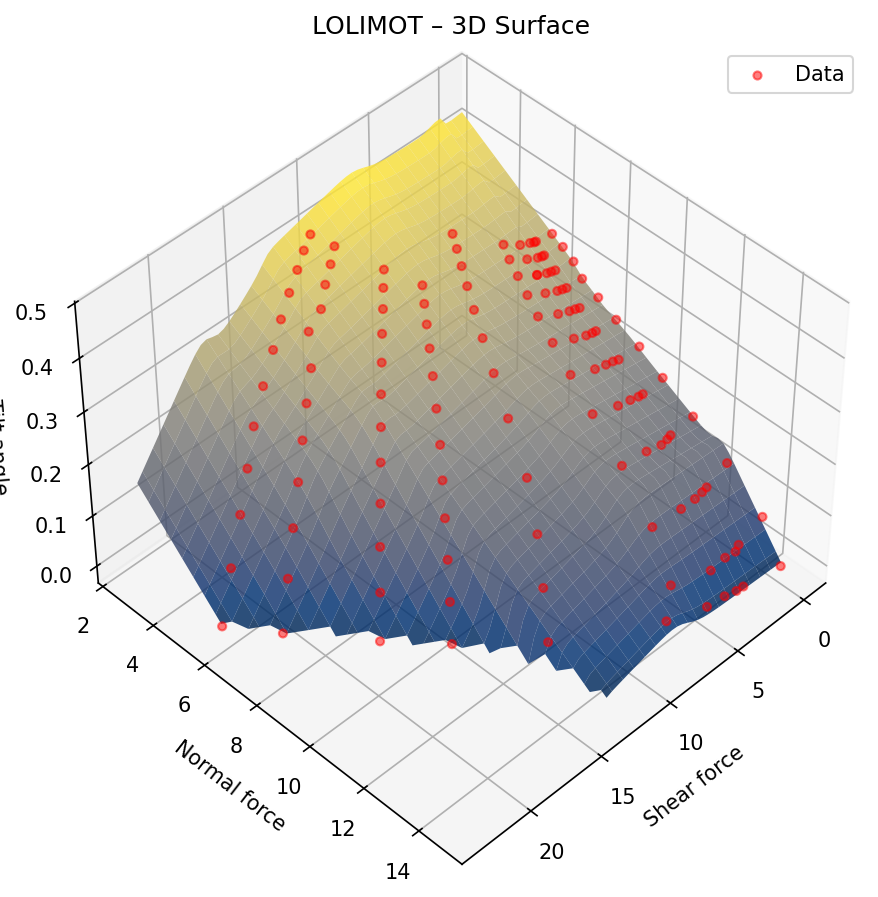
\includegraphics[width=\textwidth]{surface_lolimot.png}
  \caption{Antwortfl\"{a}che (LOLIMOT)}
  \label{fig:surface_lolimot}
\end{subfigure}
\hfill
\begin{subfigure}[b]{0.62\textwidth}
  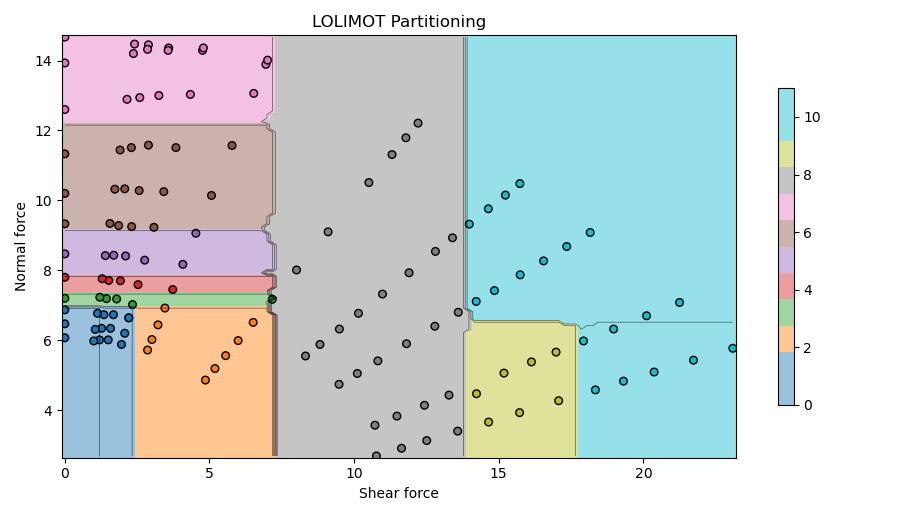
\includegraphics[width=\textwidth]{partition_lolimot.png}
  \caption{Partitionierungskarte (achsenparallel)}
  \label{fig:partition_lolimot}
\end{subfigure}
\caption{LOLIMOT: Links die 3D-Vorhersagefl\"{a}che, rechts die Partitionierungskarte.
Die achsenparallelen Trennlinien sind f\"{u}r LOLIMOT charakteristisch -- bei diagonal
orientierten Datenstrukturen entstehen typische Treppenstufen-M\"{u}ster, die mehr
Bl\"{a}tter erfordern als oblique Splits.}
\label{fig:lolimot_combined}
\end{figure}

\section{St\"{a}rken und Schw\"{a}chen von LOLIMOT}

\begin{table}[H]
\centering
\caption{St\"{a}rken und Schw\"{a}chen von LOLIMOT}
\label{tab:lolimot_pros_cons}
\begin{tabular}{p{6.5cm}p{6.5cm}}
\toprule
\textbf{St\"{a}rken} & \textbf{Schw\"{a}chen} \\
\midrule
Hohe Transparenz durch achsenparallele Regionen. & Treppenstufen-Problem bei schr\"{a}gen Grenzen. \\
Robustes, stabiles Lernverfahren. & Keine diagonalen Trennlinien. \\
Einfache Kommunikation des Modells. & Geringere Effizienz bei gekoppelten Eingaben. \\
Geringe Rechenkosten. & Extrapolation \"{u}ber lokale Netze datenabh\"{a}ngig. \\
\bottomrule
\end{tabular}
\end{table}

% ============================================================
\chapter{HILOMOT -- Hierarchical Local Model Tree}
% ============================================================

\section{Einf\"{u}hrung und Motivation}

HILOMOT (\emph{Hierarchical Local Model Tree}) ist eine Erweiterung von LOLIMOT, die von Nelles
vorgeschlagen wurde \cite{nelles2001}. Die entscheidende Neuerung ist die Zulassung
\textbf{oblique Splits} -- Trennhyperebenen mit beliebiger Orientierung im Eingangsraum.

\begin{merkbox}
HILOMOT enth\"{a}lt LOLIMOT als Spezialfall: Wenn alle Trennrichtungen auf Einheitsvektoren
$\mathbf{e}_d$ beschr\"{a}nkt werden, reduziert sich HILOMOT exakt auf LOLIMOT.
\end{merkbox}

Der Vorteil oblique Splits: Wenn die Grenze zwischen zwei Betriebsbereichen im
Kennfeld \emph{diagonal} verl\"{a}uft, kann LOLIMOT sie nur durch viele achsenparallele
Schnitte ann\"{a}hern. HILOMOT kann sie direkt mit \emph{einer} schr\"{a}gen Trennebene erfassen
-- mit deutlich weniger Bl\"{a}ttern.

\section{Oblique Splits: Mathematische Grundlage}
\label{sec:hilomot_oblique}

Ein HILOMOT-Split verwendet die allgemeine Hyperebenengleichung:
\begin{equation}
\mathbf{w}^T\mathbf{z} + b = 0
\label{eq:oblique_hyperplane}
\end{equation}
mit beliebigem Normalenvektor $\mathbf{w} \in \mathbb{R}^n$ und Bias $b \in \mathbb{R}$.

Die zugeh\"{o}rige Sigmoid-G\"{u}ltigkeitsfunktion:
\begin{equation}
\Psi(\mathbf{z}) = \frac{1}{1 + \exp\!\left(\dfrac{\kappa}{\rho}\,(\mathbf{w}^T\mathbf{z}+b)\right)}
\end{equation}

Trennhyperebene unterteilt den Eingangsraum in zwei Halbr\"{a}ume:
\begin{itemize}
\item $\mathbf{w}^T\mathbf{z} + b < 0$: linker Teilbaum (Gewicht $\Psi \to 1$),
\item $\mathbf{w}^T\mathbf{z} + b > 0$: rechter Teilbaum (Gewicht $\Psi \to 0$).
\end{itemize}

\section{Baumstruktur}

HILOMOT organisiert die Partitionierung als Bin\"{a}rbaum. Jeder innere Knoten enth\"{a}lt die
Trennparameter $(\mathbf{w}, b, \rho)$, jedes Blatt die lokalen Modellparameter
$\boldsymbol{\theta}_i$:
\begin{center}
\begin{verbatim}
          [Knoten_1: w1, b1, rho1]
         /                        \
[Knoten_2: w2, b2, rho2]      Blatt_3: theta3
     /           \
Blatt_1: theta1  Blatt_2: theta2
\end{verbatim}
\end{center}

\section{Algorithmus: HILOMOT Tree Growing}
\label{sec:hilomot_algorithm}

Das Trainingsverfahren folgt dem greedy Wachstumsrahmen von LOLIMOT, erweitert um die
Optimierung der Split-Richtung \cite{nelles2001}:

\begin{enumerate}
\item \textbf{Initialisierung:} Wie LOLIMOT (ein Blatt).
\item \textbf{Fehlerbestimmung und Auswahl des schlechtesten Blatts.}
\item \textbf{Split-Kandidaten generieren:}
      \begin{itemize}
      \item Alle achsenparallelen Richtungen $\mathbf{e}_1, \ldots, \mathbf{e}_n$.
      \item Falls \texttt{oblique=True}: zus\"{a}tzlich die erste Hauptkomponente (PCA-Richtung)
            der gewichteten Kovarianzmatrix des schlechtesten Blatts.
      \end{itemize}
\item \textbf{Kontinuierliche Winkeloptimierung} (2D): Optimaler Winkel $\theta^*$:
      \begin{equation}
      \theta^* = \arg\min_{\theta \in [0, \pi)}
                 \mathrm{MSE}\!\left(\mathbf{y},\hat{\mathbf{y}}(\theta)\right),
      \quad \mathbf{w}(\theta) = [\cos\theta,\, \sin\theta]^T
      \label{eq:hilomot_angle_opt}
      \end{equation}
\item \textbf{Besten Split ausw\"{a}hlen und Baum aktualisieren.}
\item \textbf{WLS f\"{u}r neue Bl\"{a}tter.}
\item \textbf{Abbruchkriterium pr\"{u}fen.}
\end{enumerate}

\begin{hinweisbox}
Die PCA-basierte Initialisierung der Splitrichtung ist ein zentraler Unterschied zu LOLIMOT.
Sie liefert einen guten Startpunkt f\"{u}r die Winkeloptimierung und verbessert typischerweise
die L\"{o}sungsqualit\"{a}t.
\end{hinweisbox}

\section{Demanded Membership Value}

Der Parameter \texttt{demanded\_membership\_value} ($\mu_{\min}$) legt fest, ab welchem
G\"{u}ltigkeitswert ein Datenpunkt f\"{u}r die WLS-Sch\"{a}tzung eines Blatts verwendet wird:
\begin{equation}
\mathcal{D}_i^{\text{aktiv}} = \left\{ k \mid \Phi_i(\mathbf{z}_k) \geq \mu_{\min} \right\}
\end{equation}

Zu kleine Werte: Alle Datenpunkte beeinflussen alle Bl\"{a}tter -- entspricht globalem Modell.
Zu gro\ss{}e Werte: Nur sehr nahe Datenpunkte -- Risiko schlecht konditionierter WLS-Systeme.

\section{Visualisierungen: Antwortfl\"{a}che und Partitionierungskarte}

\begin{figure}[H]
\centering
\begin{subfigure}[b]{0.34\textwidth}
  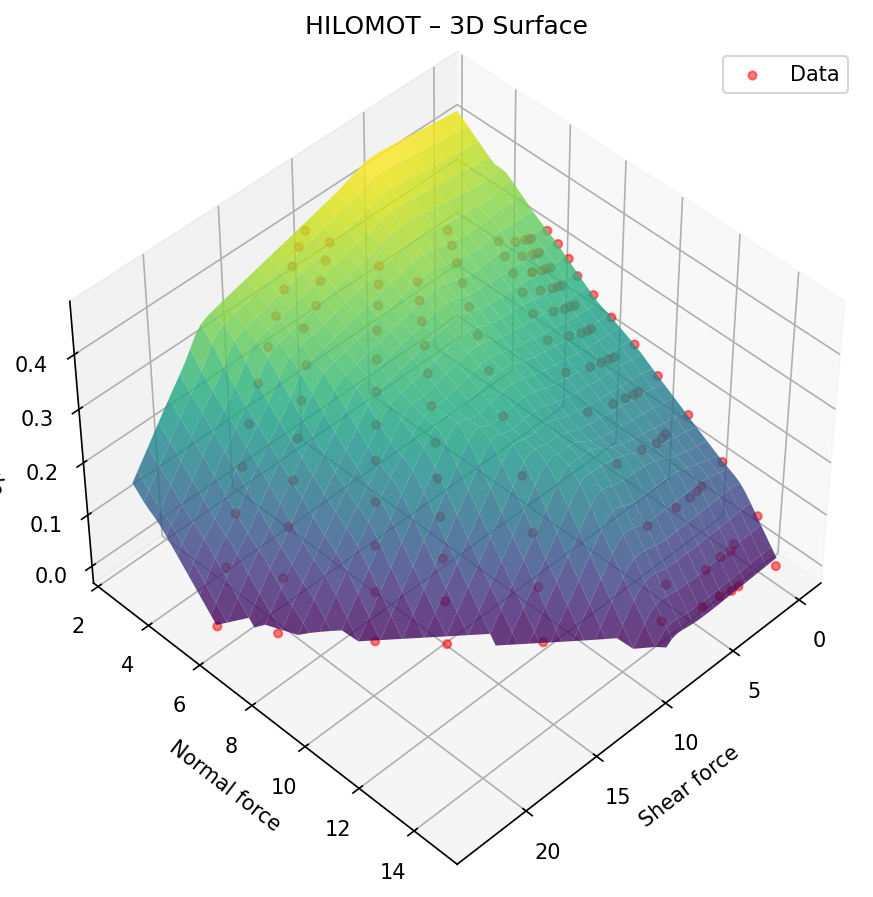
\includegraphics[width=\textwidth]{surface_hilomot.png}
  \caption{Antwortfl\"{a}che (HILOMOT)}
  \label{fig:surface_hilomot}
\end{subfigure}
\hfill
\begin{subfigure}[b]{0.62\textwidth}
  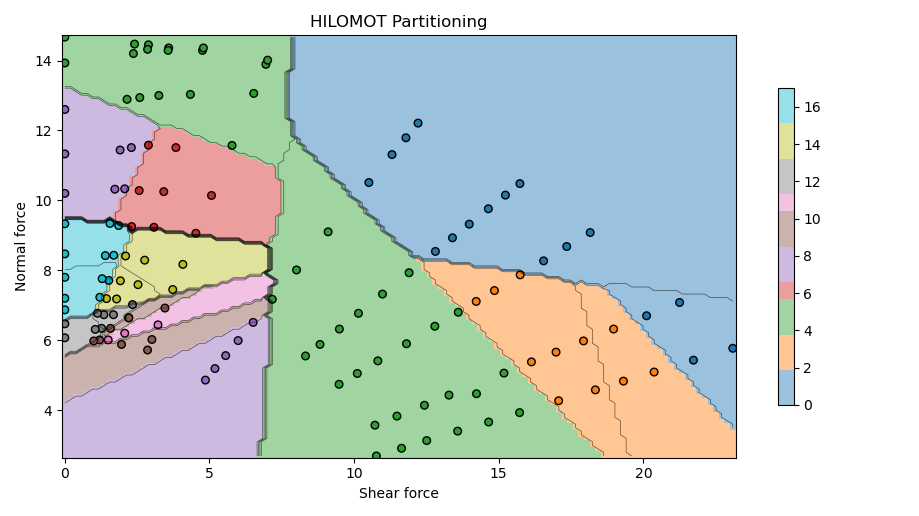
\includegraphics[width=\textwidth]{partition_hilomot.png}
  \caption{Partitionierungskarte (oblique)}
  \label{fig:partition_hilomot}
\end{subfigure}
\caption{HILOMOT: Links die 3D-Vorhersagefl\"{a}che, rechts die Partitionierungskarte. Jede Farbe
entspricht einem dominanten lokalen Modell; die Linien zeigen die Trennhyperebenen. Oblique
(schr\"{a}ge) Trennlinien sind f\"{u}r HILOMOT charakteristisch und erm\"{o}glichen eine effizientere
Beschreibung diagonaler Strukturen als achsenparallele Schnitte.}
\label{fig:hilomot_combined}
\end{figure}

\section{Hyperparameter von HILOMOT}

\begin{table}[H]
\centering
\caption{Wichtige Hyperparameter von HILOMOT im L2ML-Fitting-Tool}
\label{tab:hilomot_params}
\begin{tabular}{p{4.5cm}p{2cm}p{7cm}}
\toprule
\textbf{Parameter} & \textbf{Typ} & \textbf{Beschreibung} \\
\midrule
\texttt{max\_leafs} & int & Max. Bl\"{a}tteranzahl (Modellkomplexit\"{a}t). \\
\texttt{min\_samples\_per\_leaf} & int & Mindestanzahl Datenpunkte je Blatt. \\
\texttt{smoothness} ($\rho$) & float & Steilheitsparameter der Sigmoid-Splits. \\
\texttt{demanded\_membership} & float & Mindest-G\"{u}ltigkeitswert f\"{u}r WLS-Sch\"{a}tzung. \\
\texttt{oblique} & bool & Aktiviert oblique Splits (PCA + Winkeloptimierung). \\
\bottomrule
\end{tabular}
\end{table}

\section{St\"{a}rken und Schw\"{a}chen von HILOMOT}

\begin{table}[H]
\centering
\caption{St\"{a}rken und Schw\"{a}chen von HILOMOT}
\label{tab:hilomot_pros_cons}
\begin{tabular}{p{6.5cm}p{6.5cm}}
\toprule
\textbf{St\"{a}rken} & \textbf{Schw\"{a}chen} \\
\midrule
Oblique Splits f\"{u}r effiziente Partitionierung bei gekoppelten Eing\"{a}ngen. & Training aufw\"{a}ndiger als LOLIMOT. \\
Lokale lineare Modelle physikalisch interpretierbar. & Greedy Wachstum ohne Globaloptimalit\"{a}tsgarantie. \\
Oft weniger Bl\"{a}tter als LOLIMOT bei gleicher Genauigkeit. & Empfindlicher bei stark verrauschten Daten. \\
Glatte Vorhersagefl\"{a}che durch Sigmoid-\"{U}berg\"{a}nge. & \\
Dedizierter Parameterexport f\"{u}r Echtzeitsysteme. & \\
\bottomrule
\end{tabular}
\end{table}

% ============================================================
\chapter{MLP -- Multilayer Perceptron}
% ============================================================

\section{Einf\"{u}hrung und historischer Hintergrund}

Das \emph{Multilayer Perceptron} (MLP) ist die klassische Variante des vollst\"{a}ndig verbundenen,
vorw\"{a}rtsgerichteten neuronalen Netzes. Die theoretischen Grundlagen gehen auf McCulloch \& Pitts
(1943) und Rosenblatt (1958) zur\"{u}ck; der entscheidende Durchbruch war die Entwicklung des
Backpropagation-Algorithmus durch Rumelhart, Hinton und Williams (1986)
\cite{rumelhart1986, goodfellow2016, haykin2009}.

Im L2ML-Fitting-Tool wird \texttt{MLPRegressor} aus scikit-learn verwendet \cite{sklearn_mlp, pedregosa2011}.
MATLAB stellt \"{a}quivalente Funktionalit\"{a}t \"{u}ber die Neural Network Toolbox und
\texttt{fitrnet} (Statistics and Machine Learning Toolbox) bereit \cite{matlab_neural}.

\section{Architektur}
\label{sec:mlp_architecture}

Ein MLP mit $L$ Schichten besteht aus:
\begin{itemize}
\item einer \textbf{Eingabeschicht} ($n$ Neuronen),
\item $L{-}1$ \textbf{versteckten Schichten} mit je $H_l$ Neuronen,
\item einer \textbf{Ausgabeschicht} (1 Neuron f\"{u}r Regression).
\end{itemize}

Vorw\"{a}rtsberechnung zwischen Schicht~$l$ und~$l{+}1$:
\begin{equation}
\mathbf{h}^{(l+1)} = \sigma\!\left(W^{(l)}\mathbf{h}^{(l)} + \mathbf{b}^{(l)}\right)
\label{eq:mlp_forward}
\end{equation}
mit Gewichtsmatrix $W^{(l)} \in \mathbb{R}^{H_{l+1} \times H_l}$ und Bias-Vektor
$\mathbf{b}^{(l)} \in \mathbb{R}^{H_{l+1}}$. Die Ausgabe ohne Aktivierung:
\begin{equation}
\hat{y} = W^{(L)}\mathbf{h}^{(L)} + b^{(L)}
\label{eq:mlp_output}
\end{equation}

\section{Aktivierungsfunktionen}

Die Nichtlinearit\"{a}t des MLP entsteht durch die Aktivierungsfunktion $\sigma$.
Tabelle~\ref{tab:activation_functions} zeigt g\"{a}ngige Optionen.

\begin{table}[H]
\centering
\caption{Aktivierungsfunktionen f\"{u}r MLPs (Auswahl)}
\label{tab:activation_functions}
\begin{tabular}{p{2.5cm}p{5.5cm}p{2.5cm}p{3.0cm}}
\toprule
\textbf{Name} & \textbf{Formel} & \textbf{Bereich} & \textbf{Eigenschaft} \\
\midrule
Sigmoid     & $1/(1+e^{-x})$              & $(0,1)$      & Glatt, vanishing gradient \\
Tanh        & $(e^x-e^{-x})/(e^x+e^{-x})$ & $(-1,1)$    & Nullzentriert \\
ReLU        & $\max(0, x)$                 & $[0,\infty)$ & Einfach, kein vanishing gradient \\
Leaky ReLU  & $\max(0.01x, x)$             & $\mathbb{R}$ & Verhindert dying ReLU \\
ELU         & $x$ f\"{u}r $x>0$; $\alpha(e^x{-}1)$ sonst & $\mathbb{R}$ & Glatter \"{U}bergang \\
\bottomrule
\end{tabular}
\end{table}

\section{Backpropagation und Gradientenabstieg}
\label{sec:backpropagation}

Das MLP minimiert die Verlustfunktion MSE durch iterativen Gradientenabstieg
\cite{rumelhart1986, goodfellow2016}:
\begin{equation}
\mathcal{L}(\boldsymbol{\theta}) = \frac{1}{N}\sum_{i=1}^N (y_i - \hat{y}_i)^2
\end{equation}

\textbf{Backpropagation} berechnet effizient $\nabla_{\boldsymbol{\theta}} \mathcal{L}$
mittels der Kettenregel. Der einfache Gradientenabstieg:
\begin{equation}
\boldsymbol{\theta}^{(t+1)} = \boldsymbol{\theta}^{(t)} - \eta \nabla_{\boldsymbol{\theta}} \mathcal{L}
\end{equation}

In scikit-learn ist auch \textbf{Adam} verf\"{u}gbar \cite{sklearn_mlp}, der adaptive Lernraten
pro Parameter verwendet:
\begin{equation}
\boldsymbol{\theta}^{(t+1)} =
\boldsymbol{\theta}^{(t)} - \frac{\eta}{\sqrt{\hat{v}^{(t)}}+\epsilon}\,\hat{m}^{(t)}
\end{equation}
mit laufendem Mittelwert $\hat{m}$ (erster Moment) und Varianzsch\"{a}tzung $\hat{v}$
(zweiter Moment).

\section{Regularisierung: L2-Bestrafung}

Die regularisierte Verlustfunktion:
\begin{equation}
\mathcal{L}_{\text{reg}} = \mathcal{L} + \frac{\alpha}{2}\sum_l \lVert W^{(l)}\rVert_F^2
\label{eq:mlp_regularization}
\end{equation}
$\alpha$ (\texttt{alpha}) gro\ss{}: kleinere Gewichte, weniger Overfitting, mehr Bias.

\section{Universelle Approximationseigenschaft}

Ein MLP mit einer einzigen versteckten Schicht und gen\"{u}gend Neuronen kann jede stetige
Funktion auf einem kompakten Definitionsbereich beliebig genau approximieren
(\emph{Universal Approximation Theorem}, Cybenko 1989) \cite{bishop2006, goodfellow2016}.

\begin{hinweisbox}
Die universelle Approximationseigenschaft garantiert \emph{Existenz} einer L\"{o}sung, aber nicht
\emph{Auffindbarkeit} durch Gradientenabstieg. In der Praxis sind tiefere Netze mit weniger
Neuronen je Schicht oft effizienter.
\end{hinweisbox}

\section{Antwortfl\"{a}che}

\begin{figure}[H]
\centering
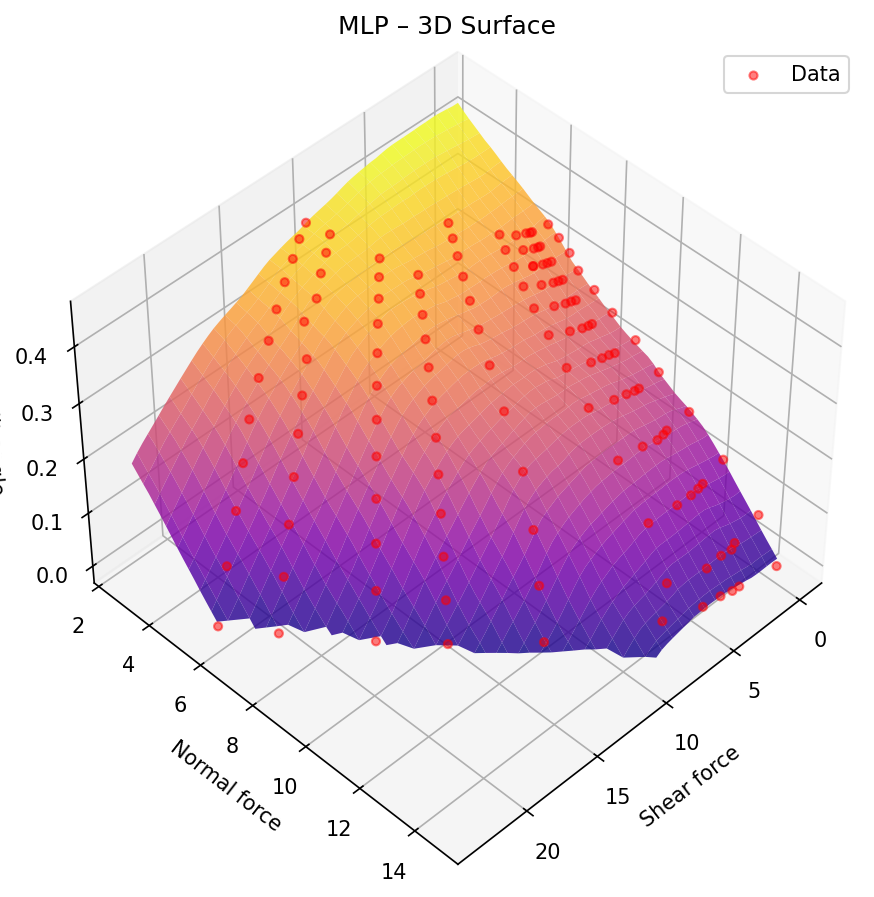
\includegraphics[width=0.68\textwidth]{surface_mlp.png}
\caption{Modellierte Antwortfl\"{a}che (MLP). Das neuronale Netz approximiert die Zielfunktion
als globale, glatte nichtlineare Abbildung ohne sichtbare Partitionierungsstruktur. Die
Oberfl\"{a}che ist weicher und weniger strukturiert als bei HILOMOT/LOLIMOT.}
\label{fig:surface_mlp}
\end{figure}

\section{Hyperparameter von MLPRegressor}

\begin{table}[H]
\centering
\caption{Wichtige Hyperparameter des MLP im L2ML-Fitting-Tool (\texttt{MLPRegressor})}
\label{tab:mlp_params}
\begin{tabular}{p{4.5cm}p{2cm}p{7cm}}
\toprule
\textbf{Parameter} & \textbf{Typ} & \textbf{Beschreibung} \\
\midrule
\texttt{hidden\_layer\_sizes} & tuple & Neuronen je Schicht, z.\,B.\ \texttt{(100, 50)}. \\
\texttt{activation} & str & \texttt{'relu'} (Standard), \texttt{'tanh'}, \texttt{'logistic'}. \\
\texttt{alpha} & float & L2-Regularisierungsparameter. \\
\texttt{learning\_rate\_init} & float & Initialer Wert der Lernrate. \\
\texttt{max\_iter} & int & Max. Trainingsiterationen (Epochen). \\
\texttt{solver} & str & \texttt{'adam'} (Standard), \texttt{'sgd'}, \texttt{'lbfgs'}. \\
\bottomrule
\end{tabular}
\end{table}

\section{St\"{a}rken und Schw\"{a}chen von MLP}

\begin{table}[H]
\centering
\caption{St\"{a}rken und Schw\"{a}chen des MLP}
\label{tab:mlp_pros_cons}
\begin{tabular}{p{6.5cm}p{6.5cm}}
\toprule
\textbf{St\"{a}rken} & \textbf{Schw\"{a}chen} \\
\midrule
Sehr hohe funktionale Flexibilit\"{a}t. & Geringe Interpretierbarkeit (Black Box). \\
Starke Approximation beliebiger Nichtlinearit\"{a}ten. & Sensitiv auf Hyperparameter. \\
Gute Fit-Werte bei ausreichenden Daten. & Overfitting-Risiko bei kleinen Datens\"{a}tzen. \\
Skaliert gut mit Datenmenge. & Keine Unsicherheitsquantifizierung. \\
Breite Tooling-Unterst\"{u}tzung. & Skalierung der Eingaben essentiell. \\
\bottomrule
\end{tabular}
\end{table}

% ============================================================
\chapter{SVR -- Support Vector Regression}
% ============================================================

\section{Einf\"{u}hrung und historischer Hintergrund}

Support Vector Machines wurden Anfang der 1990er Jahre von Vapnik entwickelt und f\"{u}r
Regression als \emph{Support Vector Regression} (SVR) adaptiert
\cite{vapnik1998, drucker1997, smola2004}. SVR geh\"{o}rt zu den leistungsf\"{a}higsten Verfahren
f\"{u}r mittlere Datens\"{a}tze.

MATLAB bietet SVR \"{u}ber \texttt{fitrsvm} im Statistics and Machine Learning Toolbox
\cite{matlab_svr}. Im L2ML-Fitting-Tool wird scikit-learn's \texttt{SVR} eingesetzt
\cite{sklearn_svr, pedregosa2011}.

\section{Das $\varepsilon$-insensitive Verlustprinzip}
\label{sec:svr_loss}

Im Gegensatz zum MSE-Verlust definiert SVR eine \emph{$\varepsilon$-Tube} um die Vorhersage:
Fehler betragsmä\ss{}ig kleiner als $\varepsilon$ erhalten Verlust~0:
\begin{equation}
L_\varepsilon(y, \hat{y}) = \max\!\left(0,\, |y - \hat{y}| - \varepsilon\right)
\label{eq:eps_loss}
\end{equation}

Nur Datenpunkte au\ss{}erhalb der $\varepsilon$-Tube (die \emph{Support Vectors}) bestimmen das
Modell -- eine sparsame Darstellung.

\section{Prim\"{a}res Optimierungsproblem}

Das prim\"{a}re SVR-Problem (lineare Variante) \cite{vapnik1998, smola2004}:
\begin{equation}
\min_{\mathbf{w}, b, \xi, \xi^*}
\;\frac{1}{2}\lVert\mathbf{w}\rVert^2 + C\sum_{i=1}^N\bigl(\xi_i + \xi_i^*\bigr)
\label{eq:svr_primal}
\end{equation}
unter Nebenbedingungen:
\begin{align}
y_i - \mathbf{w}^T\mathbf{x}_i - b &\leq \varepsilon + \xi_i \\
\mathbf{w}^T\mathbf{x}_i + b - y_i &\leq \varepsilon + \xi_i^* \\
\xi_i, \xi_i^* &\geq 0
\end{align}
$C > 0$ ist der Regularisierungsparameter; $\xi_i, \xi_i^*$ Schlupfvariablen.

\textbf{Einfluss von $C$:}
\begin{itemize}
\item Kleines $C$: viele Support Vectors erlaubt, Modell glatter (hoher Bias, geringe Varianz).
\item Gro\ss{}es $C$: wenige Ausrei\ss{}er toleriert, Modell kann komplexer werden.
\end{itemize}

\section{Duales Problem und Kernel-Trick}

Das duale Problem:
\begin{equation}
\max_{\alpha, \alpha^*} \;\;
-\frac{1}{2}\sum_{i,j}\bigl(\alpha_i-\alpha_i^*\bigr)\bigl(\alpha_j-\alpha_j^*\bigr)
K(\mathbf{x}_i,\mathbf{x}_j)
-\varepsilon\sum_i\bigl(\alpha_i+\alpha_i^*\bigr)
+\sum_i y_i\bigl(\alpha_i-\alpha_i^*\bigr)
\end{equation}

Vorhersage f\"{u}r neuen Punkt $\mathbf{x}^*$:
\begin{equation}
\hat{y}(\mathbf{x}^*) = \sum_{i\in\text{SV}} (\alpha_i - \alpha_i^*)\,K(\mathbf{x}_i, \mathbf{x}^*) + b
\end{equation}

\textbf{Kernel-Trick:} Durch $K(\mathbf{x}, \mathbf{x}') = \langle\phi(\mathbf{x}), \phi(\mathbf{x}')\rangle$
wird implizit in einen h\"{o}herdimensionalen Merkmalsraum eingebettet \cite{scholkopf2002}.

\section{RBF-Kernel}

Der am h\"{a}ufigsten verwendete Kernel f\"{u}r nichtlineare SVR:
\begin{equation}
K(\mathbf{x}, \mathbf{x}') = \exp\!\left(-\gamma\,\lVert\mathbf{x} - \mathbf{x}'\rVert^2\right)
\label{eq:rbf_kernel}
\end{equation}

$\gamma$ steuert die Reichweite des Kernels: Kleines $\gamma$ = breiter Kern, global wirkend;
gro\ss{}es $\gamma$ = schmaler Kern, lokal wirkend.

\begin{hinweisbox}
F\"{u}r die meisten Regressionsprobleme mit unbekannter Datenstruktur ist der RBF-Kernel eine
gute Standardwahl. MATLAB empfiehlt ebenfalls den RBF-Kernel als Standardoption
f\"{u}r \texttt{fitrsvm} \cite{matlab_svr}.
\end{hinweisbox}

\section{Antwortfl\"{a}che}

\begin{figure}[H]
\centering
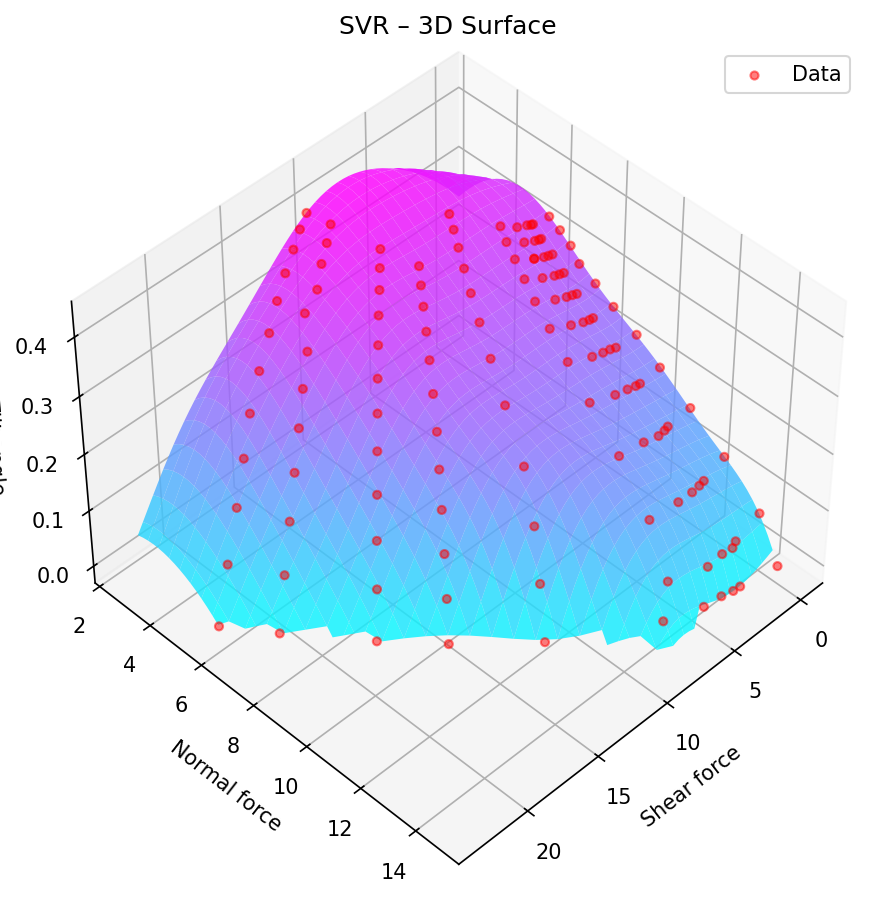
\includegraphics[width=0.68\textwidth]{surface_svr.png}
\caption{Modellierte Antwortfl\"{a}che (SVR mit RBF-Kernel). Der Kernel erm\"{o}glicht die Approxi-
mation komplexer Nichtlinearit\"{a}ten bei gleichzeitig kontrollierter Komplexit\"{a}t durch~$C$.}
\label{fig:surface_svr}
\end{figure}

\section{Hyperparameter von SVR}

\begin{table}[H]
\centering
\caption{Wichtige Hyperparameter der SVR im L2ML-Fitting-Tool}
\label{tab:svr_params}
\begin{tabular}{p{3cm}p{2cm}p{8.5cm}}
\toprule
\textbf{Parameter} & \textbf{Typ} & \textbf{Beschreibung} \\
\midrule
\texttt{C}       & float & Regularisierungsparameter. Gro\ss{}: enger Fit. Klein: glattest. \\
\texttt{gamma}   & float & RBF-Kernel-Reichweite. Gro\ss{}: lokal. Klein: global. \\
\texttt{epsilon} & float & Breite der $\varepsilon$-Tube. Klein: engere Toleranz, mehr SVs. \\
\texttt{kernel}  & str   & \texttt{'rbf'} (Standard), \texttt{'poly'}, \texttt{'sigmoid'}. \\
\bottomrule
\end{tabular}
\end{table}

\section{St\"{a}rken und Schw\"{a}chen von SVR}

\begin{table}[H]
\centering
\caption{St\"{a}rken und Schw\"{a}chen der SVR}
\label{tab:svr_pros_cons}
\begin{tabular}{p{6.5cm}p{6.5cm}}
\toprule
\textbf{St\"{a}rken} & \textbf{Schw\"{a}chen} \\
\midrule
Gute Generalisierung bei kleinen bis mittleren Datens\"{a}tzen. & Parameter schwer intuitiv einzustellen. \\
Robustes Lernprinzip durch Margin-Maximierung. & Hohe Rechenkosten f\"{u}r gro\ss{}e $N$. \\
Sparsame Darstellung durch Support Vectors. & Kein probabilistisches Ausgabeformat. \\
Guter RBF-Kernel f\"{u}r unbekannte Strukturen. & Schlechte Interpretierbarkeit. \\
\bottomrule
\end{tabular}
\end{table}

% ============================================================
\chapter{GPR -- Gaussian Process Regression}
% ============================================================

\section{Einf\"{u}hrung und historischer Hintergrund}

Gaussian Process Regression (GPR) -- auch \emph{Kriging} in der Geostatistik -- ist ein
probabilistisches, nichtparametrisches Verfahren \cite{rasmussen2006}. Im Gegensatz zu
HILOMOT/LOLIMOT, MLP und SVR gibt GPR eine \emph{vollst\"{a}ndige Wahrscheinlichkeitsverteilung}
\"{u}ber m\"{o}gliche Funktionswerte aus, also neben der Punktvorhersage auch Unsicherheitsintervalle.

MATLAB bietet GPR \"{u}ber \texttt{fitrgp} \cite{matlab_gpr}. Im L2ML-Fitting-Tool wird
scikit-learn's \texttt{GaussianProcessRegressor} verwendet \cite{sklearn_gpr, pedregosa2011}.

\section{Grundkonzept: Verteilung \"{u}ber Funktionen}

Ein \emph{Gau\ss{}scher Prozess} ist eine Verallgemeinerung der multivariaten Normalverteilung
auf Funktionen:
\begin{equation}
f(\mathbf{x}) \sim \mathcal{GP}\bigl(m(\mathbf{x}),\, k(\mathbf{x},\mathbf{x}')\bigr)
\label{eq:gp_prior}
\end{equation}
mit Mittelwertfunktion $m(\mathbf{x})$ und Kovarianzfunktion $k(\mathbf{x},\mathbf{x}')$.

F\"{u}r endlich viele Punkte $\mathbf{X}$:
\begin{equation}
\mathbf{f} \sim \mathcal{N}\!\left(\mathbf{m},\, K(\mathbf{X},\mathbf{X})\right)
\end{equation}
mit Gram-Matrix $K_{ij} = k(\mathbf{x}_i, \mathbf{x}_j)$.

\section{Kovarianzfunktionen (Kernel)}

Die Kernelwahl bestimmt die a-priori-Annahmen \"{u}ber Glattheit und Struktur der Funktion
\cite{rasmussen2006}:

\subsection{Squared Exponential (RBF) Kernel}

\begin{equation}
k_{\text{SE}}(\mathbf{x}, \mathbf{x}') = \sigma_f^2
\exp\!\left(-\frac{\lVert\mathbf{x}-\mathbf{x}'\rVert^2}{2\ell^2}\right)
\label{eq:se_kernel}
\end{equation}

$\ell$ (Length-Scale): Korrelationsreichweite; $\sigma_f^2$ (Signal-Varianz): Schwankungsbreite
der a-priori-Funktionen.

\subsection{Mat\'{e}rn-Kernel}

\begin{equation}
k_{\nu}(r) = \frac{2^{1-\nu}}{\Gamma(\nu)}
\left(\frac{\sqrt{2\nu}\,r}{\ell}\right)^\nu
K_\nu\!\left(\frac{\sqrt{2\nu}\,r}{\ell}\right)
\end{equation}
mit $r = \lVert\mathbf{x}-\mathbf{x}'\rVert$, modifizierter Bessel-Funktion $K_\nu$ und
Gl\"{a}ttegrad $\nu$. F\"{u}r $\nu \to \infty$ ergibt sich der SE-Kernel.

\subsection{Rauschterm}

\begin{equation}
k_{\text{ges}}(\mathbf{x},\mathbf{x}') = k(\mathbf{x},\mathbf{x}') + \sigma_n^2\,\delta(\mathbf{x},\mathbf{x}')
\end{equation}
mit Rauschvarianz $\sigma_n^2$ (\texttt{noise\_level}).

\section{Bayes'sche Inferenz: Posterior-Verteilung}

Gegeben Trainingsdaten $\mathcal{D} = (\mathbf{X}, \mathbf{y})$ und neuer Punkt $\mathbf{x}^*$
\cite{rasmussen2006}:
\begin{align}
\hat{f}(\mathbf{x}^*) &= \mathbf{k}_*^T\bigl(K + \sigma_n^2 I\bigr)^{-1}\mathbf{y}
\label{eq:gpr_mean} \\
\mathrm{Var}\!\left[\hat{f}(\mathbf{x}^*)\right] &= k(\mathbf{x}^*,\mathbf{x}^*)
- \mathbf{k}_*^T\bigl(K + \sigma_n^2 I\bigr)^{-1}\mathbf{k}_*
\label{eq:gpr_variance}
\end{align}
mit $\mathbf{k}_* = [k(\mathbf{x}^*, \mathbf{x}_1), \ldots, k(\mathbf{x}^*, \mathbf{x}_N)]^T$.

Der Erwartungswert (Gl.~\ref{eq:gpr_mean}) ist die Punktvorhersage; die Varianz
(Gl.~\ref{eq:gpr_variance}) quantifiziert die Vorhersageunsicherheit. Datendichte Bereiche
$\Rightarrow$ geringe Varianz; datenleere Bereiche $\Rightarrow$ gro\ss{}e Varianz.

\section{Hyperparameter-Optimierung via Marginal Likelihood}

Kernelparameter ($\ell$, $\sigma_f^2$, $\sigma_n^2$) werden durch Maximierung der
\emph{Log-Marginal-Likelihood} gesch\"{a}tzt \cite{rasmussen2006}:
\begin{equation}
\log p(\mathbf{y}|\mathbf{X}, \boldsymbol{\theta}) =
-\frac{1}{2}\mathbf{y}^T K_y^{-1} \mathbf{y}
-\frac{1}{2}\log\lvert K_y\rvert
-\frac{N}{2}\log(2\pi)
\end{equation}
mit $K_y = K + \sigma_n^2 I$. Das L2ML-Fitting-Tool f\"{u}hrt \texttt{n\_restarts\_optimizer} Neustarts
der L-BFGS-B-Optimierung durch.

\section{Antwortfl\"{a}che}

\begin{figure}[H]
\centering
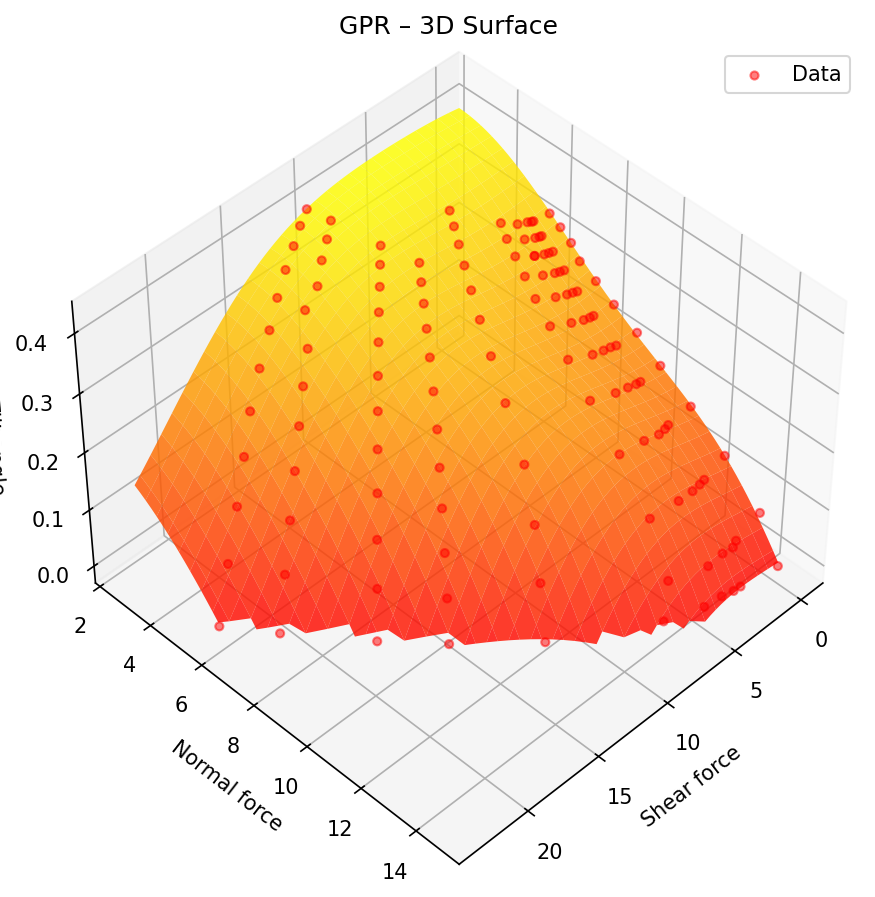
\includegraphics[width=0.68\textwidth]{surface_gpr.png}
\caption{Modellierte Antwortfl\"{a}che (GPR). Gaussian Process Regression liefert eine sehr
glatte Approximation, die eng den Trainingsdaten folgt. In datenleeren Randbereichen zieht
das Modell in Richtung der Priorfunktion.}
\label{fig:surface_gpr}
\end{figure}

\section{Hyperparameter von GaussianProcessRegressor}

\begin{table}[H]
\centering
\caption{Wichtige Hyperparameter der GPR im L2ML-Fitting-Tool}
\label{tab:gpr_params}
\begin{tabular}{p{4.5cm}p{2cm}p{7cm}}
\toprule
\textbf{Parameter} & \textbf{Typ} & \textbf{Beschreibung} \\
\midrule
\texttt{length\_scale} ($\ell$) & float & L\"{a}ngenskalierungsparameter des Kernels. \\
\texttt{noise\_level} ($\sigma_n^2$) & float & Rauschterm im Kernel (Messrauschen). \\
\texttt{n\_restarts\_optimizer} & int & Neustarts der Marginal-Likelihood-Optimierung. \\
\texttt{max\_fit\_samples} & int & Max. Datenpunkte f\"{u}r Training (Skalierungsbegrenzung). \\
\bottomrule
\end{tabular}
\end{table}

\section{St\"{a}rken und Schw\"{a}chen von GPR}

\begin{table}[H]
\centering
\caption{St\"{a}rken und Schw\"{a}chen der GPR}
\label{tab:gpr_pros_cons}
\begin{tabular}{p{6.5cm}p{6.5cm}}
\toprule
\textbf{St\"{a}rken} & \textbf{Schw\"{a}chen} \\
\midrule
Fundierte probabilistische Basis. & Kubische Rechenkosten $\mathcal{O}(N^3)$. \\
Vorhersageunsicherheit direkt verf\"{u}gbar. & Stark kernelabh\"{a}ngig. \\
Gute G\"{u}te bei kleinen Datens\"{a}tzen. & Nicht skalierbar f\"{u}r sehr gro\ss{}e $N$. \\
Kernelparameter automatisch aus Daten gesch\"{a}tzt. & Numerische Instabilit\"{a}t m\"{o}glich. \\
\bottomrule
\end{tabular}
\end{table}

% ============================================================
\chapter{L2ML-Tool}
% ============================================================

\section{L2ML-Fitting-Tool (Python)}
\label{sec:l2ml_fitting}
% ============================================================

\subsection{\"{U}berblick und Architektur}

L2ML-Fitting-Tool ist ein Python-basiertes Vergleichswerkzeug f\"{u}r f\"{u}nf Regressionsverfahren
auf einem einheitlichen Datensatz. Das Tool ist eine Portierung und Erweiterung der MATLAB
LMNTool-Toolbox \cite{matlab_lmnhelp} und verwendet f\"{u}r HILOMOT/LOLIMOT eine
Eigenimplementierung sowie f\"{u}r MLP, SVR und GPR scikit-learn \cite{pedregosa2011}.

\subsection{Datenimport und Vorverarbeitung}

CSV-Import mit Spaltenreihenfolge $y$, $x_1$, $x_2$. Nach dem Import:
\begin{itemize}
\item Pr\"{u}fung auf numerische Typen,
\item optionale Normierung auf $[0, 1]$ oder $\mathcal{N}(0,1)$,
\item 3D-Datenvorschau zur Plausibilit\"{a}tspr\"{u}fung.
\end{itemize}

\begin{figure}[H]
\centering
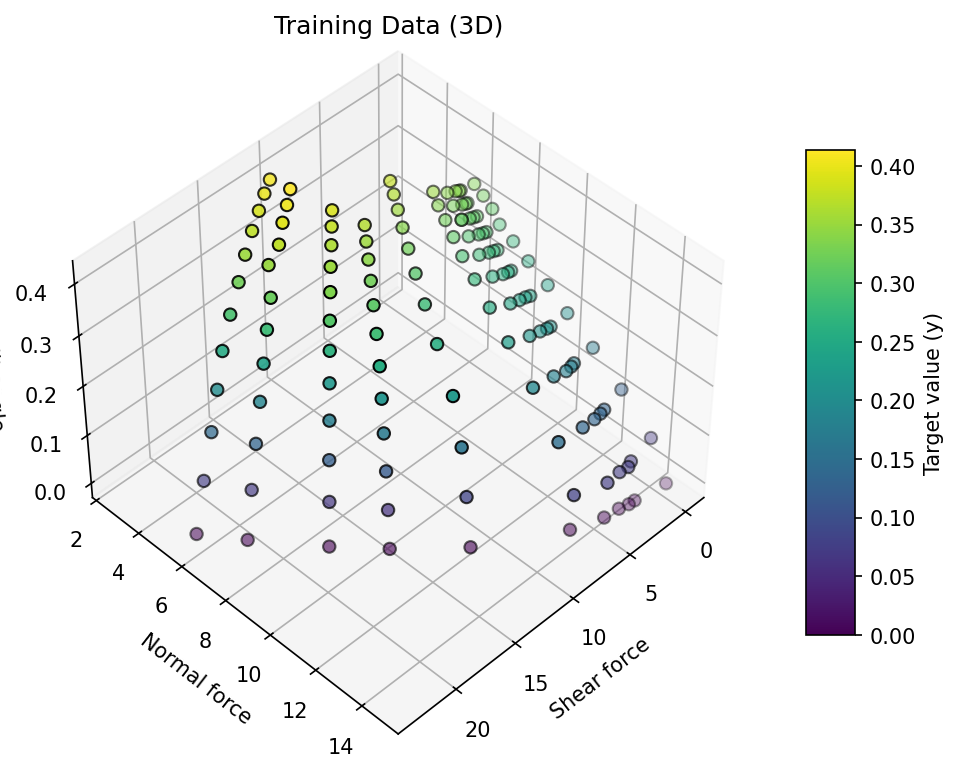
\includegraphics[width=0.65\textwidth]{training_data_3d.png}
\caption{3D-Datenvorschau im L2ML-Fitting-Tool nach dem CSV-Import. Die Visualisierung erm\"{o}glicht
eine erste visuelle Plausibilit\"{a}tspr\"{u}fung -- z.\,B.\ auf Ausrei\ss{}er, L\"{u}cken oder
unerwartete Strukturen.}
\label{fig:data_preview_tool}
\end{figure}

\subsection{Methoden-Tabs und Parametrierung}

Jeder Methoden-Tab enth\"{a}lt Eingabefelder f\"{u}r alle methodenspezifischen Hyperparameter
(vgl.\ Tab.~\ref{tab:all_params}), einen \texttt{Train}-Button und eine Statusanzeige mit
MSE, MAE, $R^2$ nach dem Training.

\begin{table}[H]
\centering
\caption{Zusammenfassung der Kernparameter aller Methoden im L2ML-Fitting-Tool}
\label{tab:all_params}
\begin{tabular}{p{2.2cm}p{11cm}}
\toprule
\textbf{Methode} & \textbf{Typische Kernparameter} \\
\midrule
HILOMOT & \texttt{max\_leafs}, \texttt{min\_samples\_per\_leaf}, \texttt{smoothness},
          \texttt{demanded\_membership\_value}, \texttt{oblique} \\
LOLIMOT & Analoge Baumparameter ohne oblique \\
MLP     & \texttt{hidden\_layer\_sizes}, \texttt{alpha}, \texttt{learning\_rate\_init},
          \texttt{max\_iter} \\
SVR     & \texttt{C}, \texttt{gamma}, \texttt{epsilon} \\
GPR     & \texttt{length\_scale}, \texttt{noise\_level}, \texttt{n\_restarts\_optimizer},
          \texttt{max\_fit\_samples} \\
\bottomrule
\end{tabular}
\end{table}

\subsection{Training und Bewertungslogik}

\textbf{Trainingsmodi:}
\begin{itemize}
\item \textbf{Einzeltraining:} Nur die aktive Methode wird trainiert.
\item \textbf{Train-All:} Alle f\"{u}nf Methoden nacheinander mit aktuellen Parametern.
\end{itemize}

\textbf{Bewertungslogik} (vier normierte Kriterien):
\begin{equation}
\text{Score}_{\text{gesamt}} = w_1 S_{\text{Acc}} + w_2 S_{\text{Ext}} +
                                w_3 S_{\text{Eff}} + w_4 S_{\text{Int}},
\quad \sum w_i = 1
\end{equation}

Zus\"{a}tzlich werden berechnet: Extrapolation Linearity, Numerical Efficiency,
Interpretability Score.

\begin{figure}[H]
\centering
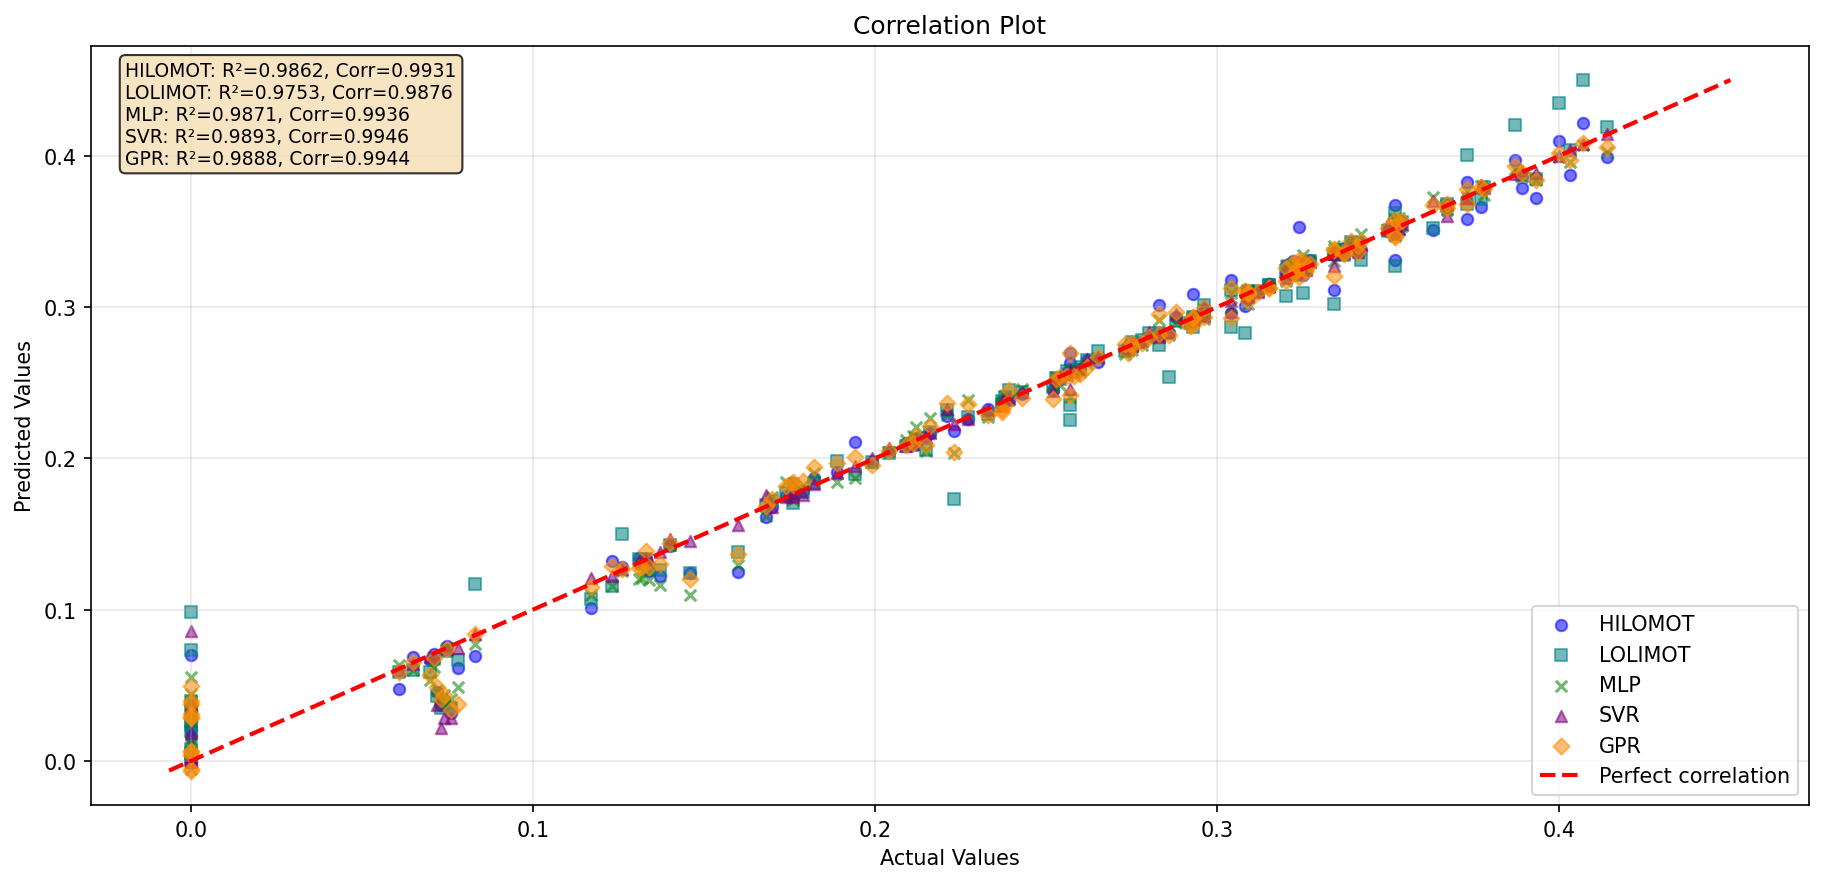
\includegraphics[width=0.68\textwidth]{correlation_plot.png}
\caption{Korrelationsplot im L2ML-Fitting-Tool: gemessene Zielwerte $y$ vs.\ Modellvorhersage $\hat{y}$.
Gute Regression: Punkte nahe der Winkelhalbierenden. Systematische Abweichungen zeigen Modellbias.}
\label{fig:correlation_plot}
\end{figure}

\begin{hinweisbox}
Die normalisierte Vergleichsansicht skaliert jedes Kriterium auf $[0,1]$, wobei 1 jeweils
dem besten Methodenwert entspricht.
\end{hinweisbox}

\subsection{Visualisierungen}

\begin{figure}[H]
\centering
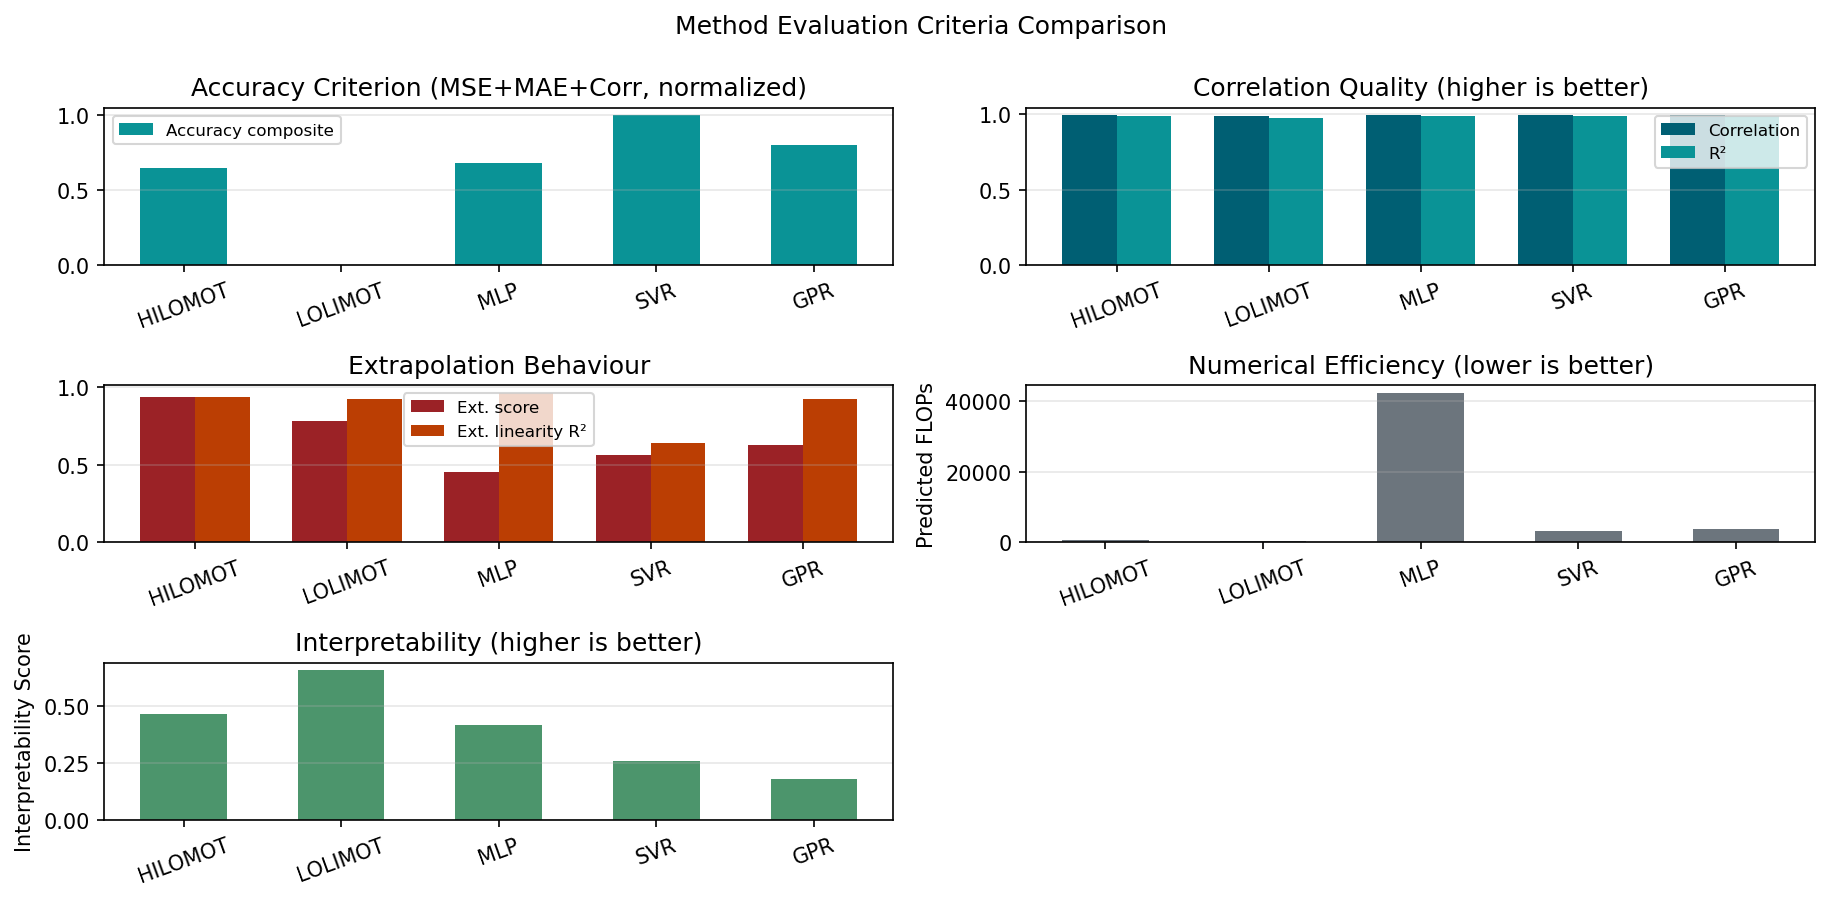
\includegraphics[width=0.68\textwidth]{evaluation_bars.png}
\caption{Evaluation Bars: absoluter Vergleich aller f\"{u}nf Methoden \"{u}ber die Kriterien
Accuracy, Extrapolation Linearity, Numerical Efficiency und Interpretability.}
\label{fig:eval_bars}
\end{figure}

\begin{figure}[H]
\centering
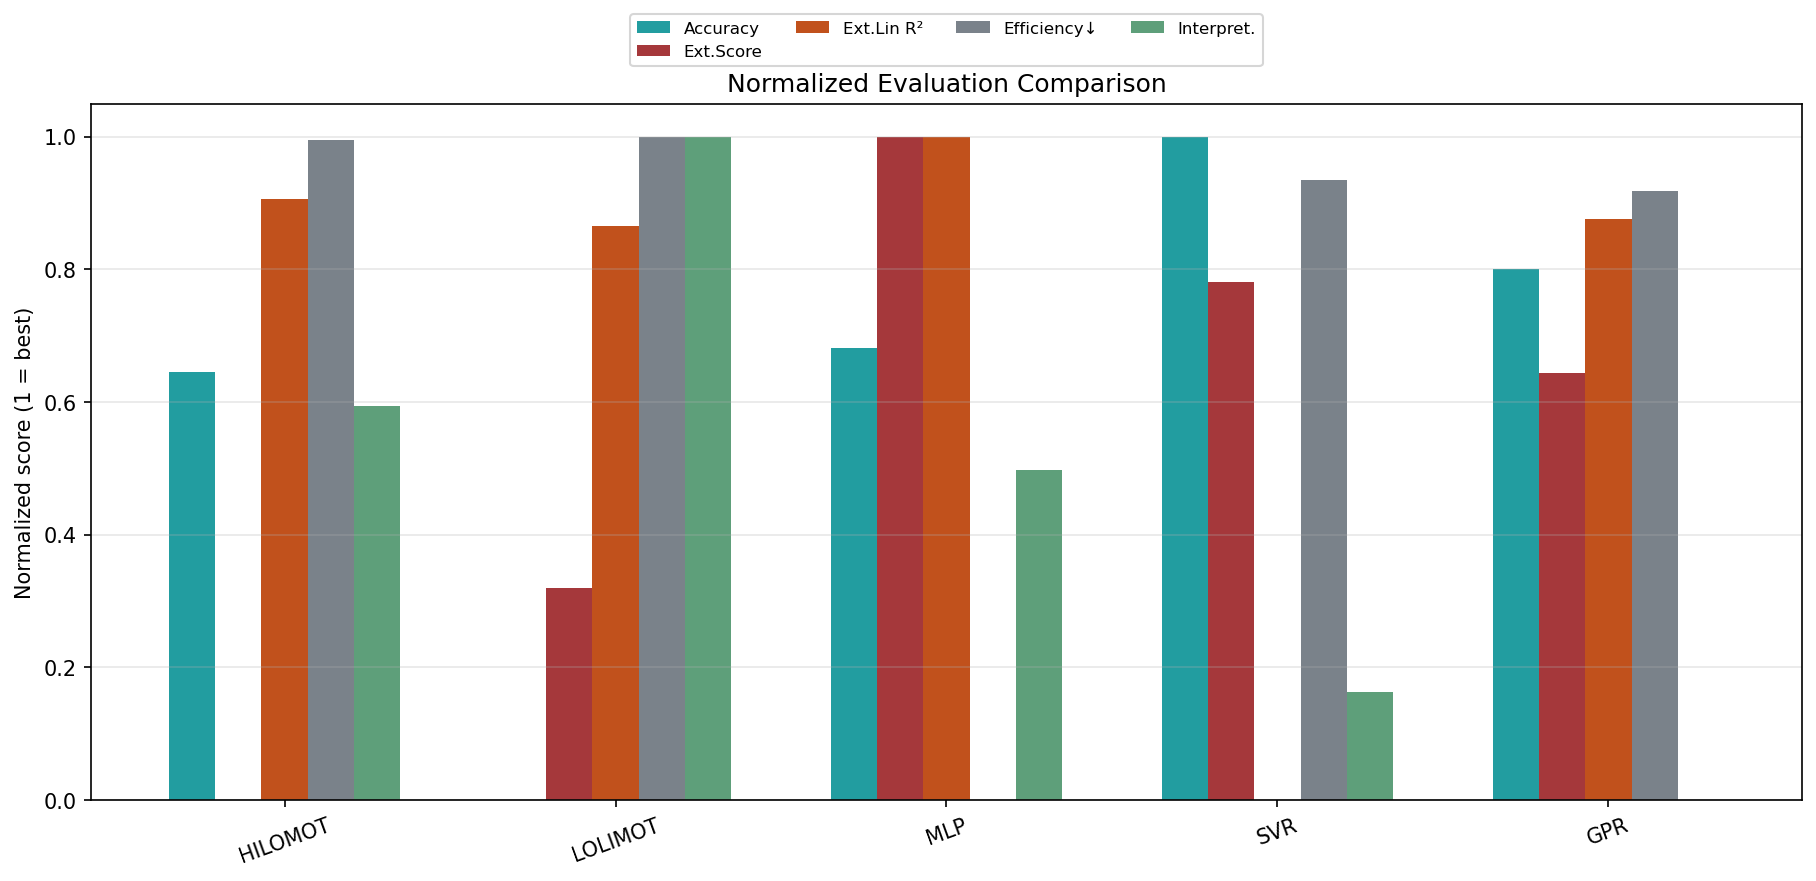
\includegraphics[width=0.68\textwidth]{evaluation_bars_normalized.png}
\caption{Normalisierte Evaluation Bars: Jedes Kriterium ist auf $[0,1]$ skaliert, wobei 1
der jeweils besten Methode entspricht. Diese Darstellung macht relative St\"{a}rken/Schw\"{a}chen
auf einen Blick erkennbar.}
\label{fig:eval_bars_norm}
\end{figure}

\begin{figure}[H]
\centering
\begin{subfigure}[b]{0.32\textwidth}
  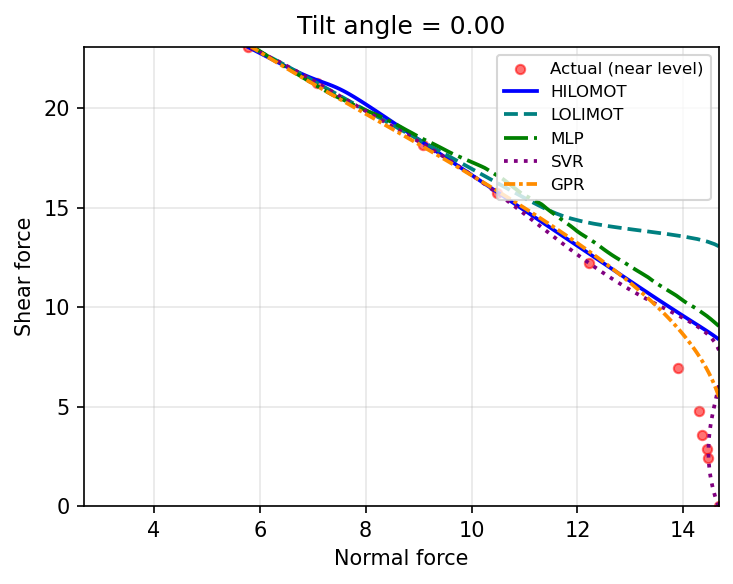
\includegraphics[width=\textwidth]{tilt_cut_01.png}
  \caption{Schnitt 1}
\end{subfigure}
\hfill
\begin{subfigure}[b]{0.32\textwidth}
  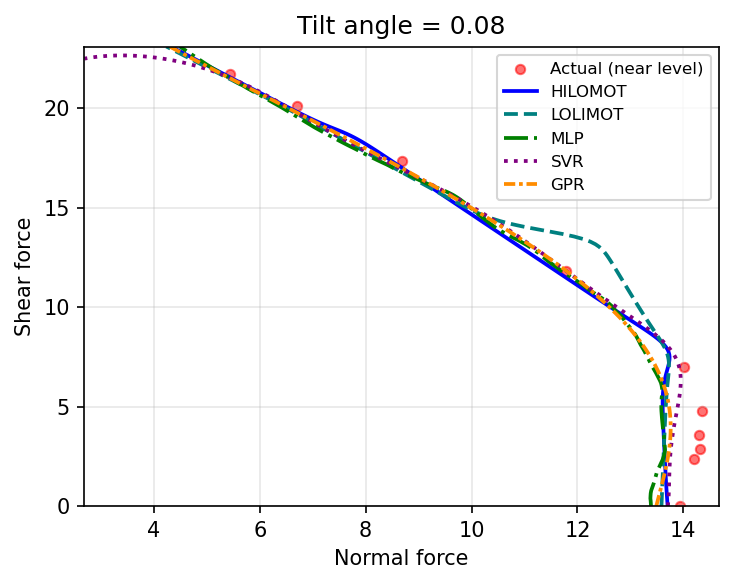
\includegraphics[width=\textwidth]{tilt_cut_02.png}
  \caption{Schnitt 2}
\end{subfigure}
\hfill
\begin{subfigure}[b]{0.32\textwidth}
  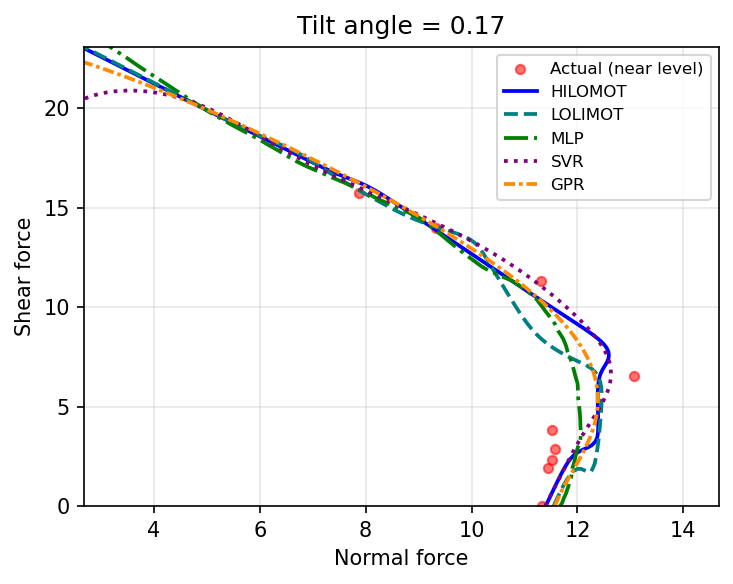
\includegraphics[width=\textwidth]{tilt_cut_03.png}
  \caption{Schnitt 3}
\end{subfigure}\\[6pt]
\begin{subfigure}[b]{0.32\textwidth}
  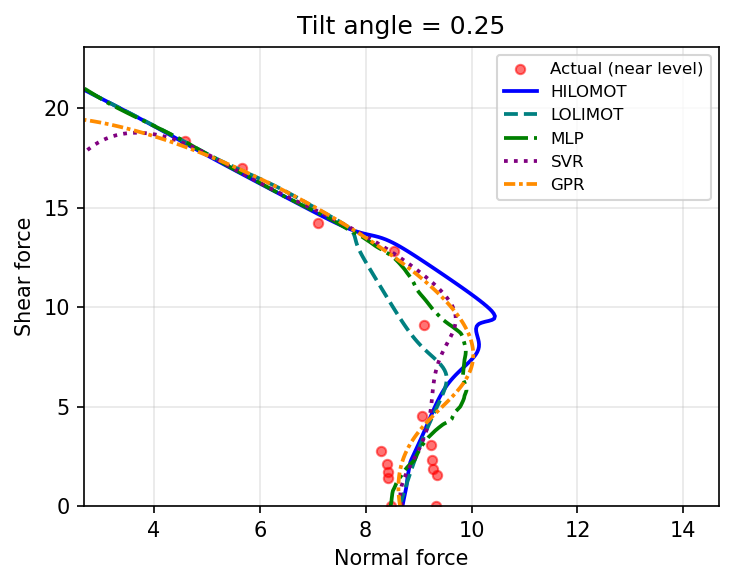
\includegraphics[width=\textwidth]{tilt_cut_04.png}
  \caption{Schnitt 4}
\end{subfigure}
\hfill
\begin{subfigure}[b]{0.32\textwidth}
  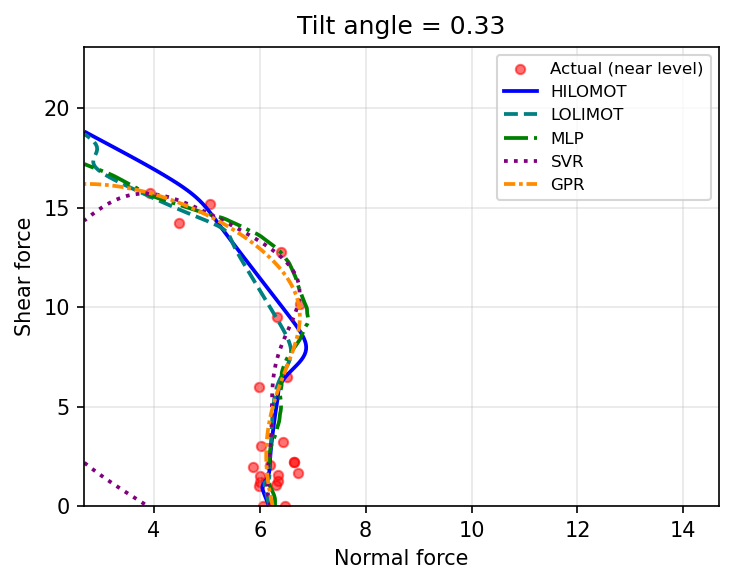
\includegraphics[width=\textwidth]{tilt_cut_05.png}
  \caption{Schnitt 5}
\end{subfigure}
\hfill
\begin{subfigure}[b]{0.32\textwidth}
  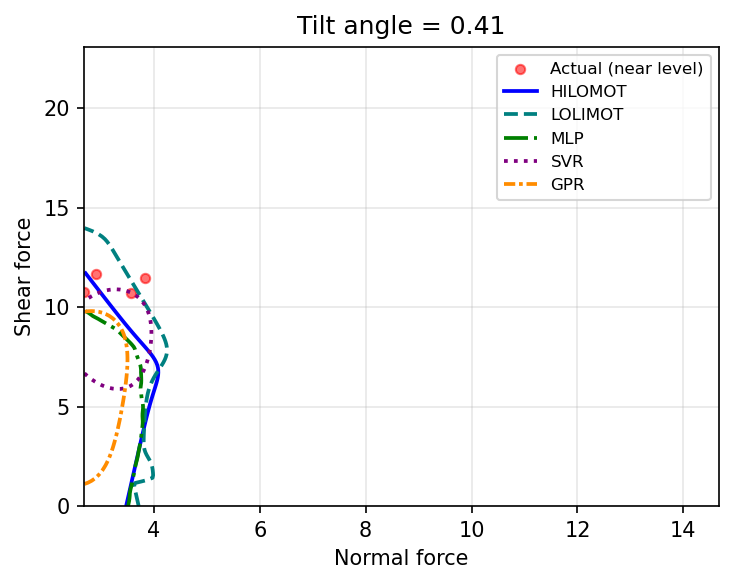
\includegraphics[width=\textwidth]{tilt_cut_06.png}
  \caption{Schnitt 6}
\end{subfigure}
\caption{Tilt Angle Cuts: Schnitte durch die modellierten Antwortfl\"{a}chen bei sechs verschiedenen
Normalkraft-Niveaus ($x_2 = \mathrm{const}$). Alle f\"{u}nf Methoden werden je Schnitt \"{u}berlagert
dargestellt. Abweichungen zwischen den Kurven zeigen methodenspezifische Unterschiede in
Interpolation und Extrapolationsverhalten.}
\label{fig:tilt_cuts}
\end{figure}

\subsection{Report- und Datenexport}

Exportformate:
\begin{itemize}
\item \textbf{JSON:} Vollst\"{a}ndige Modellparameter aller trainierten Methoden.
\item \textbf{CSV:} Vorhersagen $\hat{y}$ aller Methoden.
\item \textbf{TXT:} Lesbare Zusammenfassung der G\"{u}tekriterien.
\item \textbf{LaTeX/PDF:} Automatisch generierter Bericht mit Tabellen und Abbildungen.
\end{itemize}

F\"{u}r HILOMOT/LOLIMOT: Dedizierter Parameterexport mit allen Baumknoten f\"{u}r direkte
Einbettung in Echtzeitsysteme (z.\,B.\ MATLAB/Simulink).

% ============================================================
\section{MeinWindowLMNTool (MATLAB)}

\subsection{\"{U}berblick und Einordnung}

\begin{figure}[H]
\centering
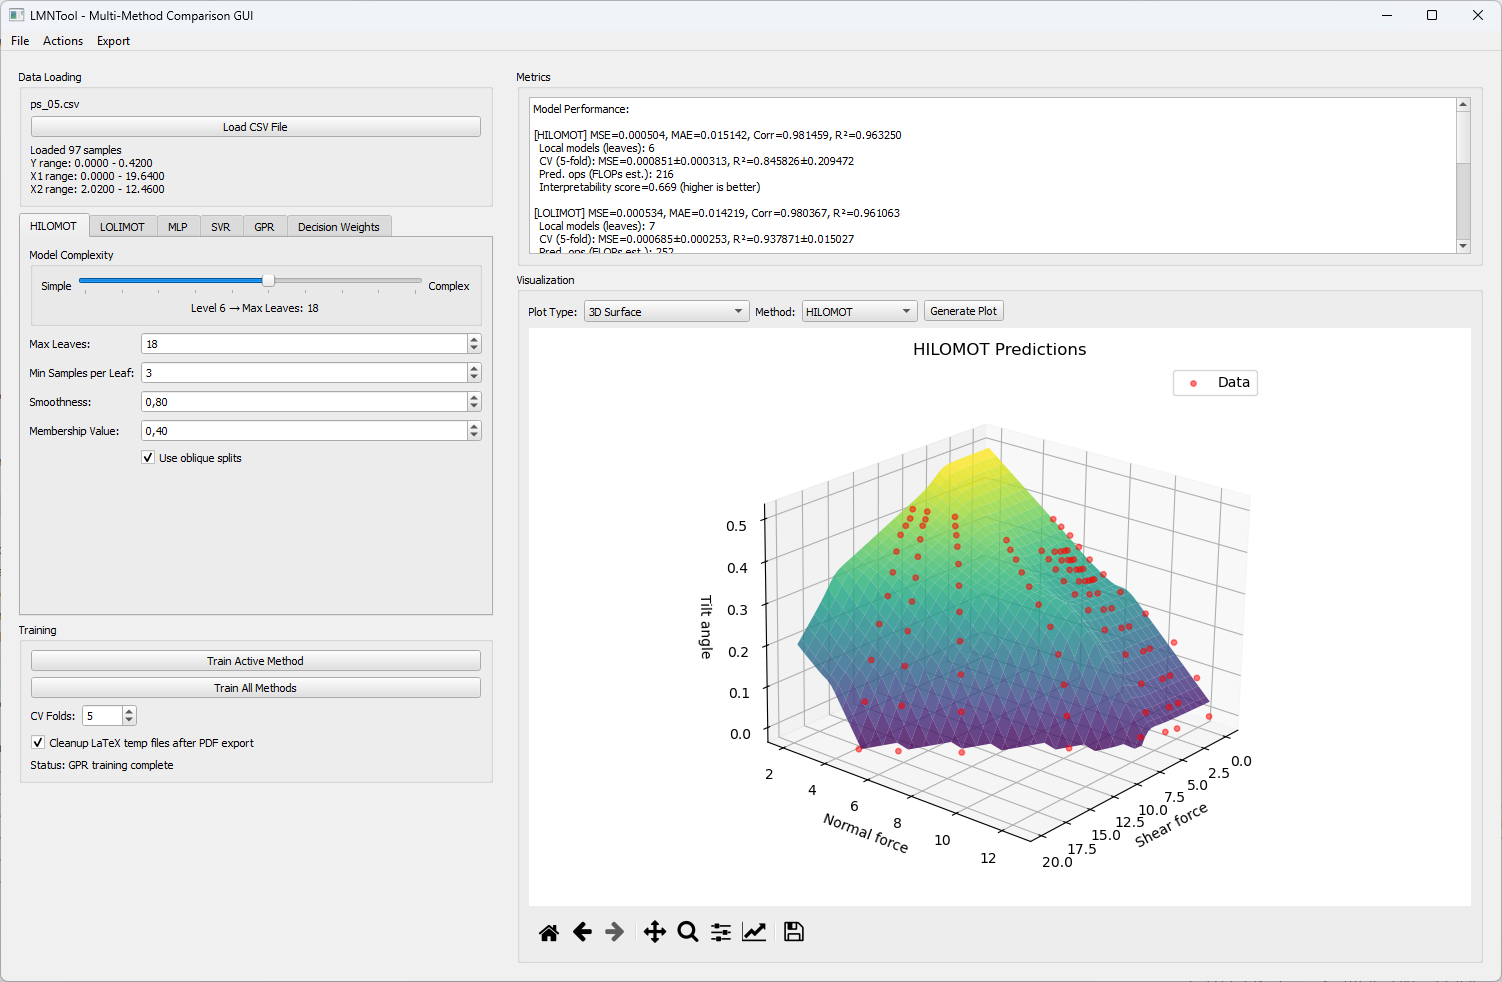
\includegraphics[width=0.92\textwidth]{MeinWindowLMNTool.png}
\caption{Hauptfenster von MeinWindowLMNTool: Steuerbereich (links) mit Methoden-\,/\,Parameterwahl,
Plotbereich (Mitte/rechts) mit 3D-Antwortfl\"{a}che und Partitionierungskarte sowie
Ergebnisbereich (unten) mit G\"{u}tekennzahlen und Exportbuttons.}
\label{fig:meinwindow_gui}
\end{figure}

\emph{MeinWindowLMNTool} ist eine interaktive, MATLAB-basierte Benutzeroberfl\"{a}che
f\"{u}r die Identifikation nichtlinearer Systeme mittels lokaler Modellnetze.
Sie baut direkt auf der MATLAB LMNTool-Toolbox (Version~1.5.2.1) der Universit\"{a}t
Siegen auf \cite{matlab_lmnhelp, matlab_lmn} und kapselt deren Kernfunktionalit\"{a}t
-- HILOMOT- und LOLIMOT-Training, Visualisierung sowie Parameterexport -- in einer
\emph{App-Designer}-Anwendung mit einer einzigen, \"{u}bersichtlichen Fensteroberfl\"{a}che.

\begin{merkbox}
\textbf{Einordnung:} W\"{a}hrend das \emph{L2ML-Fitting-Tool} (Abschnitt~\ref{sec:l2ml_fitting}) ein
Python-basiertes Vergleichswerkzeug f\"{u}r f\"{u}nf Regressionsverfahren ist, fokussiert
\emph{MeinWindowLMNTool} vollst\"{a}ndig auf HILOMOT und LOLIMOT im MATLAB-\"{O}kosystem.
Es richtet sich prim\"{a}r an Anwender, die bereits mit MATLAB vertraut sind oder eine
enge Integration mit Simulink/Control-Toolboxen ben\"{o}tigen.
\end{merkbox}

\begin{table}[H]
\centering
\caption{Gegen\"{u}berstellung: MeinWindowLMNTool vs.\ L2ML-Fitting-Tool}
\label{tab:tools_vergleich}
\begin{tabular}{p{4.0cm}p{5.2cm}p{5.2cm}}
\toprule
\textbf{Merkmal} & \textbf{MeinWindowLMNTool} & \textbf{L2ML-Fitting-Tool} \\
\midrule
Sprache / Plattform & MATLAB (App Designer) & Python (tkinter/matplotlib) \\
Unterst\"{u}tzte Methoden & HILOMOT, LOLIMOT & HILOMOT, LOLIMOT, MLP, SVR, GPR \\
Zielgruppe & MATLAB-Nutzer, Simulink-Integration & Plattform\"{u}bergreifend, Open-Source \\
Lizenz & MATLAB-Lizenz erforderlich & Python, kostenlos \\
Export & \texttt{.mat}, JSON, Text & JSON, CSV, TXT, LaTeX/PDF \\
Unsicherheitsangabe & Nein & Nur \"{u}ber GPR \\
\bottomrule
\end{tabular}
\end{table}

\subsection{Programmaufbau und Startvoraussetzungen}
\label{sec:meinwindow_start}

\textbf{Voraussetzungen:}
\begin{itemize}
\item MATLAB R2020b oder neuer (App Designer erst ab R2016a verf\"{u}gbar).
\item LMNTool-Toolbox v1.5.2.1 \cite{matlab_lmn} im MATLAB-Suchpfad (\texttt{addpath}).
\item Statistics and Machine Learning Toolbox (f\"{u}r Basisfunktionen).
\end{itemize}

\textbf{Starten der Anwendung:}

\begin{lstlisting}[language=matlab, caption={MeinWindowLMNTool starten}]
% Option 1: Direkt aus dem MATLAB Command Window
run('MeinWindowLMNTool.mlapp')

% Option 2: Doppelklick auf MeinWindowLMNTool.mlapp im
%            MATLAB Current Folder Browser
\end{lstlisting}

Nach dem Start \"{o}ffnet sich das Hauptfenster mit drei Hauptbereichen:
\begin{enumerate}
\item \textbf{Steuerbereich (links):} Dateiladen, Methoden- und Parameterwahl, Trainingsstart.
\item \textbf{Plotbereich (Mitte/rechts):} Visualisierungen (3D-Fl\"{a}che, Partitionierungskarte,
      Korrelationsplot, Schnittdarstellungen).
\item \textbf{Ergebnisbereich (unten):} G\"{u}tekennzahlen, Modellzusammenfassung und
      Exportbuttons.
\end{enumerate}

\subsection{Datenimport}
\label{sec:meinwindow_daten}

\emph{MeinWindowLMNTool} akzeptiert Datens\"{a}tze als CSV-Datei im selben 3-spaltigen Format
wie das Python-Tool:
\begin{itemize}
\item Spalte~1: Zielgr\"{o}\ss{}e $y$ (z.\,B.\ Tilt Angle),
\item Spalte~2: Eingangsgr\"{o}\ss{}e $x_1$ (z.\,B.\ Shear Force),
\item Spalte~3: Eingangsgr\"{o}\ss{}e $x_2$ (z.\,B.\ Normal Force).
\end{itemize}
Trennzeichen werden automatisch erkannt (\texttt{;}, \texttt{,}, Tab).
Zus\"{a}tzlich k\"{o}nnen Daten direkt als MATLAB-Variable (\texttt{.mat}-Datei) \"{u}bergeben werden.

\begin{lstlisting}[language=matlab, caption={Daten programmatisch laden (Skript-Modus)}]
% Trainingsdaten laden
data = readmatrix('tiltangle_data.csv');
y  = data(:,1);   % Tilt Angle
x1 = data(:,2);   % Shear Force
x2 = data(:,3);   % Normal Force

% Datenmenge X fuer L2ML-Fitting-Tool
X_train = [x1, x2];
\end{lstlisting}

Nach dem Import zeigt das Tool eine 3D-Vorschau der Rohdaten analog zu
Abbildung~\ref{fig:training_data} (Kapitel~1), um Ausrei\ss{}er und L\"{u}cken
visuell zu pr\"{u}fen, bevor das Training gestartet wird.

\subsection{Methoden- und Parameterwahl}
\label{sec:meinwindow_params}

Im Steuerbereich w\"{a}hlt der Anwender \"{u}ber ein \texttt{uiswitch}-Element zwischen
\textbf{LOLIMOT} (achsenparallel) und \textbf{HILOMOT} (oblique Splits).
Alle relevanten Hyperparameter k\"{o}nnen \"{u}ber Spinner-Felder (\texttt{uispinner})
und Checkboxen (\texttt{uicheckbox}) eingestellt werden.

\begin{table}[H]
\centering
\caption{Trainingsparameter in MeinWindowLMNTool}
\label{tab:meinwindow_params}
\begin{tabular}{p{4.5cm}p{1.8cm}p{1.5cm}p{6.5cm}}
\toprule
\textbf{Parameter} & \textbf{Typ} & \textbf{Standard} & \textbf{Beschreibung} \\
\midrule
Max Leaves & int & 15 & Maximale Bl\"{a}tteranzahl (Modellkomplexit\"{a}t). \\
Min Samples per Leaf & int & 6 & Mindestanzahl effektiver Trainingspunkte je Blatt. \\
Smoothness ($\rho$) & float & 0{,}8 & \"{U}berlappung der Sigmoid-G\"{u}ltigkeitsregionen. \\
Membership Value ($\mu^*$) & float & 0{,}4 & Mindest-G\"{u}ltigkeitswert f\"{u}r WLS-Einbeziehung. \\
Oblique Splits & bool & an & \texttt{an} = HILOMOT; \texttt{aus} = LOLIMOT. \\
Kreuzvalidierung & bool & aus & Aktiviert $k$-fache CV zur Strukturwahl. \\
$k$ (CV-Folds) & int & 5 & Anzahl der Folds bei Kreuzvalidierung. \\
\bottomrule
\end{tabular}
\end{table}

\begin{hinweisbox}
\textbf{Empfehlung:} F\"{u}r komplexe, diagonale Datenstrukturen (wie den Tilt-Angle-Datensatz)
empfiehlt sich \texttt{Oblique Splits~=~an} (HILOMOT) mit \texttt{Max Leaves~=~10--15} und
\texttt{Smoothness~=~0{,}4--0{,}8}. F\"{u}r achsenparallele, weniger gekoppelte Daten reicht
LOLIMOT oft schon mit \texttt{Max Leaves~=~8--12}.
\end{hinweisbox}

\subsection{Training}
\label{sec:meinwindow_training}

Das Training wird durch Klick auf den \textbf{Train}-Button ausgel\"{o}st.
Der Trainingsfortschritt wird in einer Fortschrittsanzeige (\texttt{uiprogressdlg}) angezeigt,
sodass die Oberfl\"{a}che w\"{a}hrend des Baumwachstums reaktionsf\"{a}hig bleibt.

Intern ruft die App die LMNTool-Kernfunktion auf:

\begin{lstlisting}[language=matlab, caption={Interner Aufruf der LMNTool-Trainingsfunktion}]
% HILOMOT-Training (intern in der App-Callback-Funktion)
opt = lmntool_options();
opt.maxLeafs       = app.MaxLeavesSpinner.Value;
opt.smoothness     = app.SmoothnessSpinner.Value;
opt.oblique        = app.ObliqueSwitchValue;
opt.minSamplesLeaf = app.MinSamplesSpinner.Value;
opt.membershipVal  = app.MembershipSpinner.Value;

model = hilomot(X_train, y, opt);   % LMNTool-Funktion
\end{lstlisting}

Nach dem Training werden direkt im Ergebnisbereich ausgegeben:

\begin{center}
\begin{tabular}{p{3.0cm}p{5.0cm}p{5.5cm}}
\toprule
\textbf{Metrik} & \textbf{Formel} & \textbf{Beschreibung} \\
\midrule
MSE & $\frac{1}{N}\sum(y_i-\hat{y}_i)^2$ & Mittlerer quadratischer Fehler \\
MAE & $\frac{1}{N}\sum|y_i-\hat{y}_i|$   & Mittlerer absoluter Fehler \\
RMSE & $\sqrt{\text{MSE}}$ & Wurzel des MSE (in Einheiten von $y$) \\
$R^2$ & $1-\mathrm{SS_{res}}/\mathrm{SS_{tot}}$ & Bestimmtheitsma\ss{} \\
Lokale Modelle & $M$ & Anzahl Bl\"{a}tter im Baum \\
Trainingszeit & $t$ [s] & Rechenaufwand des Baumwachstums \\
\bottomrule
\end{tabular}
\end{center}

\subsection{Visualisierungen}
\label{sec:meinwindow_vis}

\emph{MeinWindowLMNTool} stellt dieselben zentralen Visualisierungen bereit, die auch aus dem
Python-Tool bekannt sind (Kapitel~\ref{fig:hilomot_combined}, \ref{fig:correlation_plot}):

\begin{table}[H]
\centering
\caption{Visualisierungstypen in MeinWindowLMNTool}
\label{tab:meinwindow_vis}
\begin{tabular}{p{4.0cm}p{9.5cm}}
\toprule
\textbf{Plot-Typ} & \textbf{Beschreibung} \\
\midrule
3D Surface & Vorhersagefl\"{a}che $\hat{y}(x_1, x_2)$ mit eingebetteten Trainingspunkten
             (MATLAB \texttt{surf} + \texttt{scatter3}). \\
Partition Map & 2D-Partitionierungsplot mit eingezeichneten Trennhyperebenen und
                farbcodierten G\"{u}ltigkeitsbereichen (\texttt{pcolor}). \\
Correlation Plot & Streudiagramm $y$ vs.\ $\hat{y}$ mit Winkelhalbierender zur
                   Diagnose von Bias. \\
Tilt Cuts & Schnitte $\hat{y}(x_1)$ bei verschiedenen Niveaus $x_2 = \text{const}$.
            Direkt vergleichbar mit Abb.~\ref{fig:tilt_cuts}. \\
Validity Functions & 2D-Darstellung der einzelnen G\"{u}ltigkeitsfunktionen $\Phi_i(x_1, x_2)$
                     f\"{u}r jedes Blatt. Einzigartig unter den beiden Tools. \\
\bottomrule
\end{tabular}
\end{table}

Ein besonderes Alleinstellungsmerkmal von \emph{MeinWindowLMNTool} gegen\"{u}ber dem
Python-Pendant ist die \textbf{Validity-Function-Visualisierung}: F\"{u}r jedes Blatt~$i$
wird $\Phi_i(x_1, x_2)$ als Oberfl\"{a}che geplottet (Gleichung~\ref{eq:validity_weight}).
Diese Darstellung macht transparent, welche Datenpunkte durch welches lokale Modell
beschrieben werden -- ein wesentlicher Beitrag zur Interpretierbarkeit.

\begin{lstlisting}[language=matlab, caption={Validity-Function-Plot f\"{u}r Blatt i (Skript-Modus)}]
% Eingangsraster
[x1g, x2g] = meshgrid(linspace(min(x1),max(x1),60), ...
                       linspace(min(x2),max(x2),60));
Xgrid = [x1g(:), x2g(:)];

% Gueltigkeitsgewichte aus dem Modell abrufen
Phi = lmntool_validity(model, Xgrid);   % N_grid x M Matrix

% Blatt i plotten
figure;
surf(x1g, x2g, reshape(Phi(:,i), size(x1g)));
xlabel('Shear Force'); ylabel('Normal Force');
zlabel(['\Phi_' num2str(i)]);
title(['Gueltigkeitsfunktion -- Blatt ' num2str(i)]);
\end{lstlisting}

\subsection{Export und Integration}
\label{sec:meinwindow_export}

\emph{MeinWindowLMNTool} bietet folgende Exportoptionen:

\begin{table}[H]
\centering
\caption{Exportformate in MeinWindowLMNTool}
\label{tab:meinwindow_export}
\begin{tabular}{p{3.0cm}p{10.5cm}}
\toprule
\textbf{Format} & \textbf{Inhalt} \\
\midrule
\texttt{.mat} & Vollst\"{a}ndige MATLAB-Modellstruktur: Baum, Knotenparameter, Kappa-Werte,
                Gewichte. Direkt ladbar mit \texttt{load('model.mat')}. \\
JSON & Maschinenlesbare Beschreibung aller Baumknoten (kompatibel mit Python-Tool). \\
Text & Lesbare Zusammenfassung: Metriken, Baumstruktur, lokale Modellkoeffizienten. \\
Simulink-Block & Erzeugung eines parametrisierten \texttt{Interpreted MATLAB Function}-Blocks
                 f\"{u}r direkte Einbettung in Simulink-Modelle. \\
\bottomrule
\end{tabular}
\end{table}

\textbf{Simulink-Integration:} Der automatisch erzeugte Simulink-Block \"{u}bernimmt die gelernten
Modellparameter (Gewichte, Bias, Kappa) und bildet die LMN-Vorhersagefunktion (Gleichung~\ref{eq:lmn})
direkt in Echtzeit ab. Dies erm\"{o}glicht die direkte Nutzung des trainierten Modells
in Hardware-in-the-Loop (HiL)-Umgebungen oder Steuerger\"{a}te-Prototypen.

\begin{lstlisting}[language=matlab, caption={Modell nach Training laden und auswerten}]
% Gespeichertes Modell laden
load('hilomot_tiltangle_model.mat', 'model');

% Vorhersage fuer neuen Datenpunkt
x_new = [0.35, 1.2];   % [Shear Force, Normal Force]
y_hat = lmntool_predict(model, x_new);

fprintf('Vorhergesagter Tilt Angle: %.4f\n', y_hat);
\end{lstlisting}

\subsection{Vergleich mit dem Python L2ML-Fitting-Tool}
\label{sec:meinwindow_vergleich_python}

Beide Werkzeuge erg\"{a}nzen sich sinnvoll und richten sich an unterschiedliche Anwendergruppen:

\begin{description}
\item[MeinWindowLMNTool (MATLAB):] Ideal f\"{u}r MATLAB-Nutzer in Industrie und Hochschule,
    besonders wenn eine direkte Simulink-Integration oder Anbindung an MATLAB-Workflows
    gew\"{u}nscht ist. St\"{a}rken: Validity-Function-Visualisierung, Simulink-Export,
    native MATLAB-Datenstrukturen.

\item[L2ML-Fitting-Tool (Python):] Ideal f\"{u}r plattform\"{u}bergreifenden Einsatz und
    wenn auch MLP, SVR und GPR verglichen werden sollen. St\"{a}rken: Mehr Methoden,
    normierter Mehrkriterienscore, kostenlos nutzbar.
\end{description}

\begin{table}[H]
\centering
\caption{Funktionsumfang im Direktvergleich}
\label{tab:tools_funktionen}
\begin{tabular}{p{6.0cm}p{3.2cm}p{3.2cm}}
\toprule
\textbf{Funktion} & \textbf{MeinWindowLMNTool} & \textbf{L2ML-Fitting-Tool} \\
\midrule
HILOMOT-Training & \checkmark & \checkmark \\
LOLIMOT-Training & \checkmark & \checkmark \\
MLP / SVR / GPR & -- & \checkmark \\
3D Antwortfl\"{a}che & \checkmark & \checkmark \\
Partitionierungskarte & \checkmark & \checkmark \\
Korrelationsplot & \checkmark & \checkmark \\
Tilt Angle Cuts & \checkmark & \checkmark \\
Validity-Functions-Plot & \checkmark & -- \\
Kreuzvalidierung (GUI) & \checkmark & -- \\
Mehrkriterienscore & -- & \checkmark \\
Simulink-Export & \checkmark & -- \\
JSON-Export & \checkmark & \checkmark \\
\texttt{.mat}-Export & \checkmark & -- \\
LaTeX/PDF-Report & -- & \checkmark \\
MATLAB-Lizenz erforderlich & Ja & Nein \\
\bottomrule
\end{tabular}
\end{table}

\begin{merkbox}
F\"{u}r reine HILOMOT/LOLIMOT-Anwendungen in MATLAB-Umgebungen ist \emph{MeinWindowLMNTool}
die direktere Wahl. F\"{u}r einen \"{u}bergreifenden Methodenvergleich (inkl.\ MLP, SVR, GPR)
bietet das \emph{L2ML-Fitting-Tool} den vollst\"{a}ndigeren Rahmen.
\end{merkbox}

% ============================================================
\chapter{Vergleich der Methoden}
% ============================================================

\section{Methoden\"{u}berblick}

\begin{table}[H]
\centering
\caption{Qualitative Einordnung der f\"{u}nf Methoden nach Hauptcharakteristika}
\label{tab:methoden_uebersicht}
\begin{tabular}{p{2.5cm}p{2.8cm}p{3.5cm}p{2.5cm}p{1.8cm}}
\toprule
\textbf{Methode} & \textbf{Modelltyp} & \textbf{Kernidee} & \textbf{Interpret.} & \textbf{Unsich.} \\
\midrule
HILOMOT & Lok. Modellnetz & Oblique Splits & Hoch & Nein \\
LOLIMOT & Lok. Modellnetz & Achsenparallele Splits & Sehr hoch & Nein \\
MLP & Neuronales Netz & Globale Approx. & Gering & Nein \\
SVR & Kernel-Methode & $\varepsilon$-Margin & Mittel & Nein \\
GPR & Probabilistisch & Bayes'sche Inferenz & Mittel & Ja \\
\bottomrule
\end{tabular}
\end{table}

\section{Vergleich der Antwortfl\"{a}chen}

\begin{figure}[H]
\centering
\begin{subfigure}[b]{0.47\textwidth}
  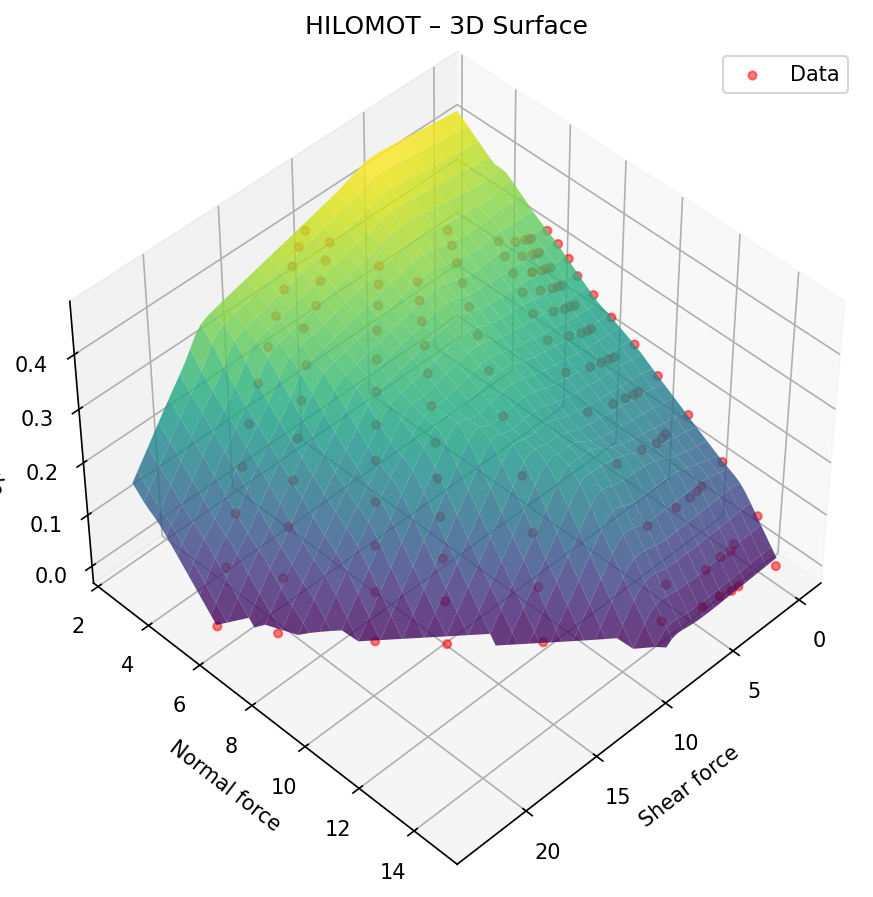
\includegraphics[width=\textwidth]{surface_hilomot.png}
  \caption{HILOMOT}
\end{subfigure}
\hfill
\begin{subfigure}[b]{0.47\textwidth}
  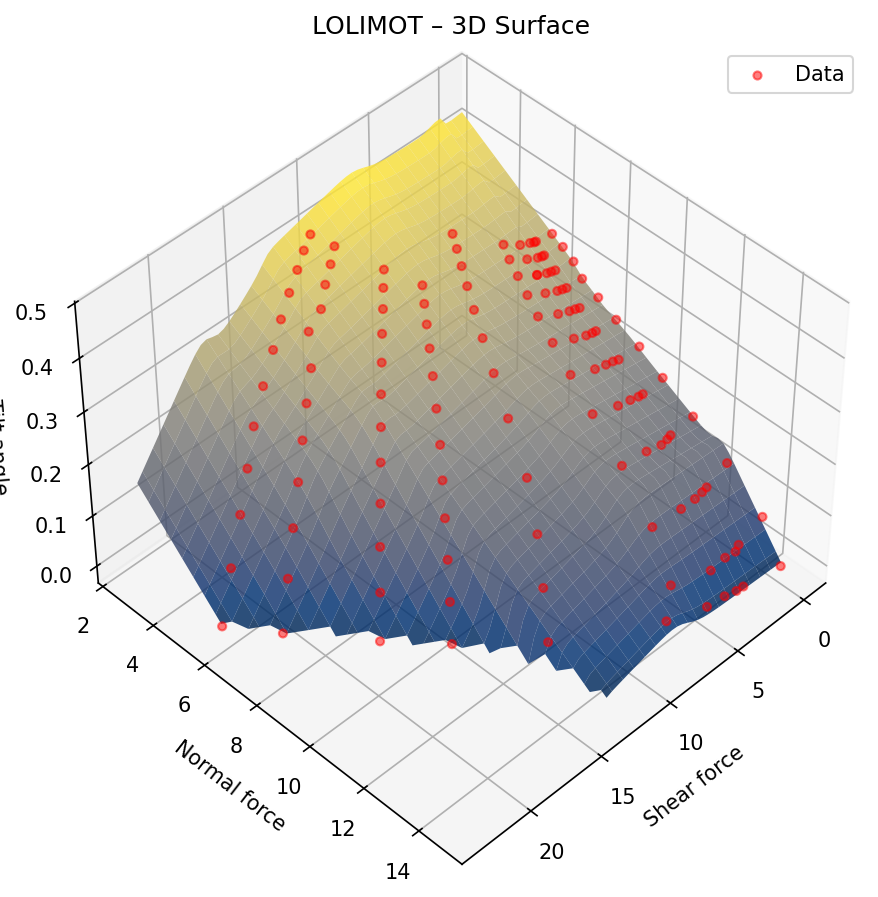
\includegraphics[width=\textwidth]{surface_lolimot.png}
  \caption{LOLIMOT}
\end{subfigure}\\[6pt]
\begin{subfigure}[b]{0.47\textwidth}
  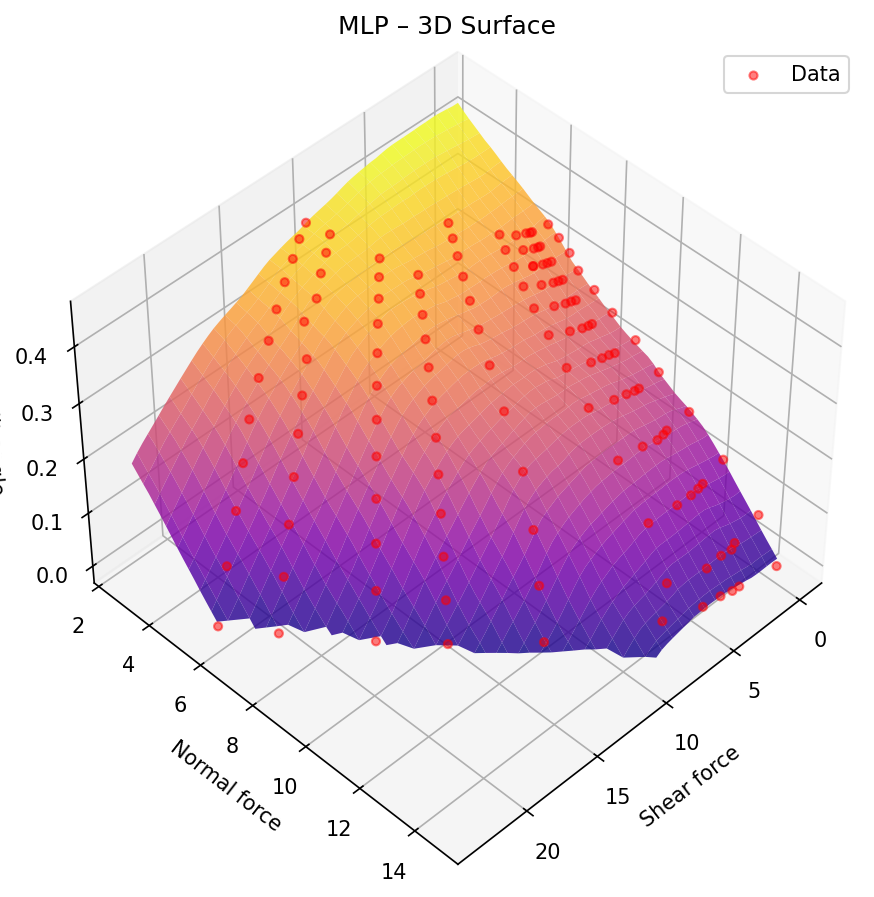
\includegraphics[width=\textwidth]{surface_mlp.png}
  \caption{MLP}
\end{subfigure}
\hfill
\begin{subfigure}[b]{0.47\textwidth}
  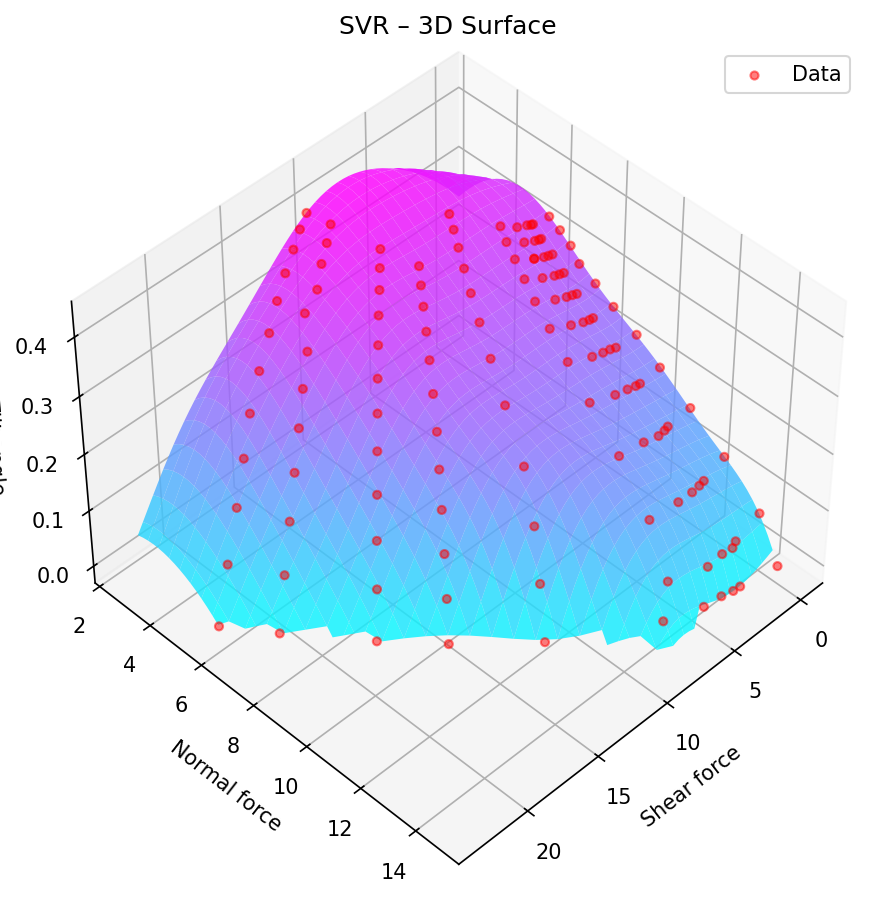
\includegraphics[width=\textwidth]{surface_svr.png}
  \caption{SVR}
\end{subfigure}\\[6pt]
\begin{subfigure}[b]{0.47\textwidth}
  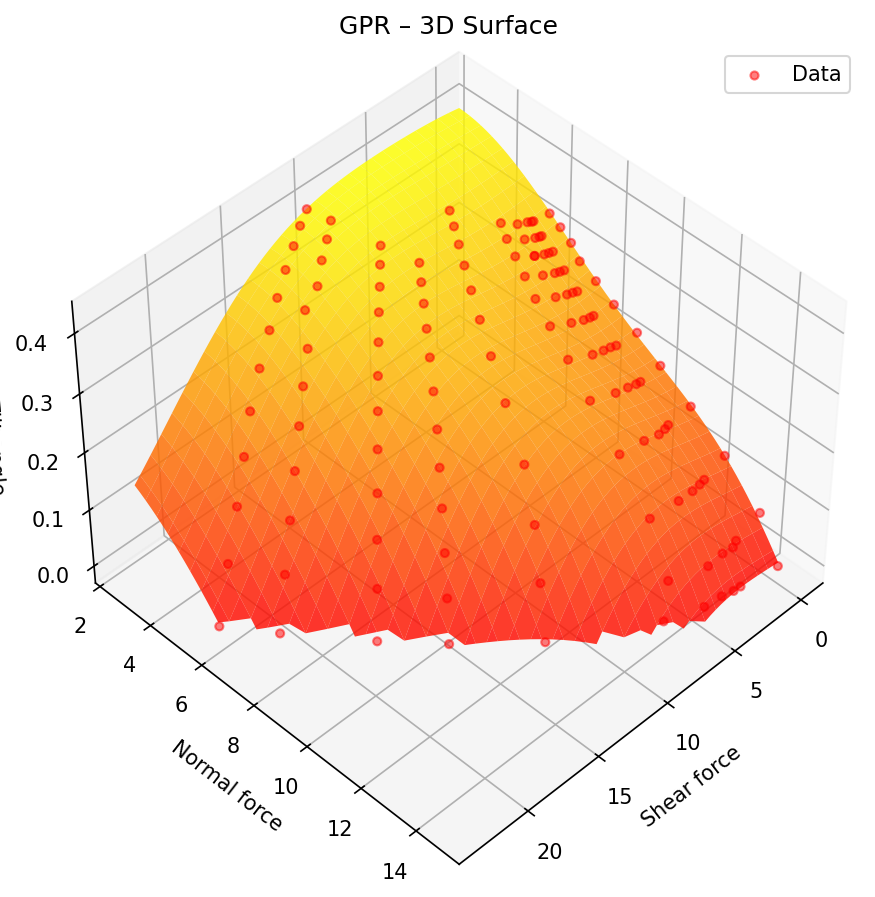
\includegraphics[width=\textwidth]{surface_gpr.png}
  \caption{GPR}
\end{subfigure}
\caption{Vergleich der modellierten Antwortfl\"{a}chen aller f\"{u}nf Methoden auf demselben
Datensatz. Qualitative Unterschiede in Gl\"{a}tte, Partitionierungsstruktur und globalem
Verhalten sind deutlich erkennbar.}
\label{fig:surfaces_comparison}
\end{figure}

\section{Tabellarischer Vergleich}

\begin{longtable}{p{2.2cm}p{5.0cm}p{5.5cm}}
\caption{Ausf\"{u}hrlicher Vergleich nach St\"{a}rken und Schw\"{a}chen}
\label{tab:methoden_vergleich} \\
\toprule
\textbf{Methode} & \textbf{St\"{a}rken} & \textbf{Schw\"{a}chen} \\
\midrule
\endfirsthead
\toprule
\textbf{Methode} & \textbf{St\"{a}rken} & \textbf{Schw\"{a}chen} \\
\midrule
\endhead
HILOMOT & Gute Balance Genauigkeit/Interpretierbarkeit; oblique Splits effizient; physikalisch plausible lokale Modelle; Parameterexport. & Mehr Parameter als globale Modelle; greedy; h\"{o}herer Tuningaufwand bei Rauschen. \\[3pt]
LOLIMOT & Sehr hohe Transparenz; robuste Modellbildung; einfach kommunizierbar; gering Rechenaufwand. & Treppenstufen bei diagonalen Grenzen; mehr Bl\"{a}tter bei gekoppelten Strukturen. \\[3pt]
MLP & Hohe Flexibilit\"{a}t; starke Approximation; gute Fit-Werte bei gen\"{u}gend Daten. & Black Box; sensitiv auf Hyperparameter; Overfitting-Risiko. \\[3pt]
SVR & Gute Generalisierung; robustes Lernprinzip; RBF-Kernel effektiv. & Parameter schwer einzustellen; hohe Laufzeiten bei gro\ss{}em $N$; keine Unsicherheit. \\[3pt]
GPR & Probabilistische Basis; Unsicherheitsquantifizierung; gut bei kleinen Datens\"{a}tzen. & $\mathcal{O}(N^3)$ Kosten; kernelabh\"{a}ngig; nicht skalierbar. \\
\bottomrule
\end{longtable}

\section{Rechenkomplexit\"{a}t}

\begin{table}[H]
\centering
\caption{Ungef\"{a}hre Rechenkomplexit\"{a}t der f\"{u}nf Methoden}
\label{tab:rechenaufwand}
\begin{tabular}{lll}
\toprule
\textbf{Methode} & \textbf{Training} & \textbf{Vorhersage} \\
\midrule
HILOMOT/LOLIMOT & $\mathcal{O}(M \cdot n \cdot N)$ & $\mathcal{O}(M)$ \\
MLP             & $\mathcal{O}(\text{Iter} \cdot N \cdot P)$ & $\mathcal{O}(P)$ \\
SVR             & $\mathcal{O}(N^2)$--$\mathcal{O}(N^3)$ & $\mathcal{O}(|\text{SV}|)$ \\
GPR             & $\mathcal{O}(N^3)$ & $\mathcal{O}(N^2)$ \\
\bottomrule
\multicolumn{3}{l}{\small $M$: Bl\"{a}tter, $n$: Dim., $N$: Datenpunkte, $P$: Netzparameter, SV: Support Vectors}
\end{tabular}
\end{table}

\section{Anwendungsempfehlungen}

\begin{enumerate}
\item \textbf{Physikalische Interpretierbarkeit:} HILOMOT oder LOLIMOT.
\item \textbf{Diagonale/schr\"{a}ge Trennstrukturen:} HILOMOT mit oblique Splits.
\item \textbf{Achsenparallele Strukturen:} LOLIMOT.
\item \textbf{Reine Vorhersageg\"{u}te, ausreichende Daten:} MLP oder SVR.
\item \textbf{Kleiner Datensatz, Unsicherheit gew\"{u}nscht:} GPR.
\item \textbf{Echtzeiteinsatz:} HILOMOT/LOLIMOT (expliziter Parameterexport).
\item \textbf{Robuste Entscheidung:} Mehrkriteriensicht und Kreuzvalidierung nutzen.
\end{enumerate}

\begin{merkbox}
Es gibt keine universell beste Methode. Die optimale Wahl h\"{a}ngt von Datencharakteristik,
Erkl\"{a}rbarkeitsanforderung, Rechenbudget, Datenmenge und Extrapolationsanforderung ab.
Der normalisierte Balkenvergleich (Abb.~\ref{fig:eval_bars_norm}) zeigt diese Abw\"{a}gungen
direkt.
\end{merkbox}

% ============================================================
\chapter{Diskussion}
% ============================================================

\section{Interpretation der Ergebnisse}

Am verwendeten Datensatz (Tilt Angle \"{u}ber Shear Force und Normal Force) zeigen alle f\"{u}nf
Methoden grundst\"{a}tzlich eine gute Approximationsleistung, was auf eine glatte, gut lernbare
Datenstruktur hindeutet. Dennoch lassen sich methodenspezifische Unterschiede beobachten:

\begin{description}
\item[HILOMOT und LOLIMOT] bilden die Struktur durch explizite Partitionierung ab. Die
    Partitionierungskarte (Abb.~\ref{fig:partition_hilomot}) zeigt klar, welche Teilmodelle
    dominieren. Bei HILOMOT sind schr\"{a}ge Trennlinien erkennbar, die auf nicht-achsenparallele
    Datenstruktur hinweisen. LOLIMOT ben\"{o}tigt f\"{u}r \"{a}hnliche Genauigkeit typischerweise
    mehr Bl\"{a}tter.

\item[MLP] liefert eine glatte, global definierte Antwortfl\"{a}che (Abb.~\ref{fig:surface_mlp})
    ohne erkennbare Partitionierungsstruktur. Das Modell ist leistungsf\"{a}hig, bietet aber
    keinen Einblick in die Datenstruktur.

\item[SVR] produziert eine glatte Oberfl\"{a}che (Abb.~\ref{fig:surface_svr}) mit Robustheit
    gegen\"{u}ber Ausrei\ss{}ern durch den $\varepsilon$-insensitiven Verlust.

\item[GPR] zeigt die glatteste Approximation (Abb.~\ref{fig:surface_gpr}) und folgt den Daten
    eng in dicht besetzten Regionen. Die Vorhersageunsicherheit ist ein wichtiger Vorteil bei
    sicherheitsrelevanten Anwendungen.
\end{description}

Die Tilt-Angle-Schnittdarstellungen (Abb.~\ref{fig:tilt_cuts}) zeigen, dass alle Methoden
im Trainingsbereich \"{a}hnliche Verl\"{a}ufe haben. Unterschiede treten prim\"{a}r in Randbereichen
und bei der Extrapolation auf.

\section{Kritische Betrachtung der Hyperparameterwahl}

Alle Methoden weisen eine erhebliche Empfindlichkeit gegen\"{u}ber der Hyperparameterwahl auf:

\begin{itemize}
\item HILOMOT/LOLIMOT: \texttt{max\_leafs} und \texttt{smoothness} entscheiden \"{u}ber den
      Bias-Varianz-Kompromiss. Zu viele Bl\"{a}tter f\"{u}hren zu Overfitting.
\item MLP: Netzgr\"{o}\ss{}e, Lernrate und $\alpha$ sind entscheidend; Grid-Search aufw\"{a}ndig.
\item SVR: $C$, $\gamma$ und $\varepsilon$ interagieren stark; MATLAB empfiehlt Kreuzvalidierung
      \cite{matlab_svr}.
\item GPR: Kernelparameter werden automatisch gesch\"{a}tzt, Anzahl Neustarts beeinflusst die
      Qualit\"{a}t.
\end{itemize}

\section{Generalisierungsf\"{a}higkeit und Extrapolation}

Das Verhalten au\ss{}erhalb des Trainingsbereichs (Extrapolation):

\begin{description}
\item[HILOMOT/LOLIMOT:] Extrapolation \"{u}ber lokale lineare Modelle in Randbereichen -- oft
    linear und physikalisch interpretierbar.
\item[MLP:] Unvorhersehbare Extrapolation; Netze k\"{o}nnen au\ss{}erhalb stark oszillieren.
\item[SVR:] RBF-Kernel l\"{a}uft au\ss{}erhalb gegen null -- unerwartete Vorhersagen m\"{o}glich.
\item[GPR:] Zieht gegen die Priorfunktion; Unsicherheit w\"{a}chst -- transparentes
    ``Nicht-Wissen''.
\end{description}

\section{Grenzen des Vergleichs}

\begin{itemize}
\item Vergleich basiert auf einem Datensatz -- andere Datens\"{a}tze k\"{o}nnen zu anderen
      Rangfolgen f\"{u}hren.
\item Hyperparameter wurden nicht systematisch per Grid-Search optimiert.
\item Tiefere neuronale Netze (CNN, Transformer) wurden nicht ber\"{u}cksichtigt.
\item Interpretierbarkeit und Extrapolation sind qualitativ eingestuft.
\end{itemize}

% ============================================================
\chapter{Zusammenfassung}
% ============================================================

\section{Wichtigste Erkenntnisse}

Diese Dokumentation hat f\"{u}nf Regressionsverfahren von den mathematischen Grundlagen bis zur
Implementierung im L2ML-Fitting-Tool ausf\"{u}hrlich beschrieben. Die zentralen Erkenntnisse:

\begin{enumerate}
\item \textbf{Lokale Modellnetze (HILOMOT, LOLIMOT)} bieten eine einzigartige Kombination aus
      nichtlinearer Approximationsleistung und physikalischer Interpretierbarkeit.

\item \textbf{HILOMOT} erreicht bei gekoppelten Daten durch oblique Splits oft bessere
      Ergebnisse mit weniger Bl\"{a}ttern als LOLIMOT.

\item \textbf{MLP} ist leistungsf\"{a}hig bei ausreichenden Daten, bietet aber wenig Einblick
      in die Datenstruktur.

\item \textbf{SVR} ist robust und gut generalisierend f\"{u}r kleine bis mittlere Datens\"{a}tze.

\item \textbf{GPR} liefert als einzige Methode Vorhersageunsicherheiten -- ein wesentlicher
      Vorteil f\"{u}r sicherheitskritische Anwendungen. Die kubische Skalierung limitiert den
      Einsatz bei gro\ss{}en Datens\"{a}tzen.

\item \textbf{Das L2ML-Fitting-Tool} erm\"{o}glicht einen direkten, reproduzierbaren Vergleich
      aller f\"{u}nf Methoden mit einheitlichen Metriken, Multi-Kriterien-Bewertung und
      interaktiven Visualisierungen.
\end{enumerate}

\section{Praktische Handlungsempfehlungen}

\begin{description}
\item[Kleiner Datensatz ($N < 500$), Unsicherheit wichtig:] GPR.
\item[Kleiner bis mittlerer Datensatz, keine Interpretierbarkeit n\"{o}tig:] SVR.
\item[Mittlerer bis gro\ss{}er Datensatz, Black Box akzeptiert:] MLP.
\item[Interpretierbarkeit wichtig, achsenparallele Strukturen:] LOLIMOT.
\item[Interpretierbarkeit wichtig, gekoppelte Eing\"{a}nge:] HILOMOT.
\item[Echtzeiteinsatz in Steuerger\"{a}t:] HILOMOT oder LOLIMOT (Parameterexport).
\end{description}

\section{Ausblick}

Zuk\"{u}nftige Erweiterungen k\"{o}nnten umfassen:
\begin{itemize}
\item Unterst\"{u}tzung h\"{o}herer Eingangsdimension ($n > 2$).
\item Integration tieferer neuronaler Netze als sechste Methode.
\item Approximate GPR (Sparse GP) f\"{u}r gro\ss{}e Datens\"{a}tze.
\item Automatische Hyperparameter-Optimierung (AutoML, Bayesian Optimization).
\item Bootstrap-Konfidenzintervalle f\"{u}r Methoden ohne probabilistischen Rahmen.
\end{itemize}

% ============================================================
% LITERATURVERZEICHNIS
% ============================================================
\printbibliography[heading=bibintoc, title={Literaturverzeichnis}]

\end{document}
